% ---------------------------------------------------------------------------
% Dual-Bottleneck Agents
%
% Batch 2: real figures and tables wired in.
%   - \includegraphics for all 12 published figures (figures/ is self-contained
%     so the paper/ directory can be uploaded to Overleaf as-is)
%   - booktabs tables built from reports/paper_data_final/tables/*.md
%   - figure captions below, table captions above (NeurIPS convention)
%   - \label on every float; cite them with \ref, never with a hard-coded number
%
% Abstract / Introduction / Section 3 are verbatim author text.
% Sections 4-8 carry no body prose yet: the prose was not supplied.
%
% Compile target: pdfLaTeX (works unchanged on Overleaf).
% ---------------------------------------------------------------------------

% ---------------------------------------------------------------------------
% NeurIPS 2026 官方模板。
% 注意：neurips_2026.sty 内部已经 RequirePackage 了 geometry / natbib / hyperref，
% 因此下面这几行不能再各自加载，否则会 option clash 直接报错。
% 原先的 \documentclass[11pt]{article} 与 \usepackage[margin=1in]{geometry}
% 会让版面变成单栏 1 英寸边距，与 NeurIPS 双栏模板冲突，已移除。
% ---------------------------------------------------------------------------
\documentclass{article}
\usepackage[preprint]{neurips_2026}

% --- encoding and fonts -----------------------------------------------------
\usepackage[utf8]{inputenc}
\usepackage[T1]{fontenc}

% --- math -------------------------------------------------------------------
\usepackage{amsmath}
\usepackage{amssymb}

% --- figures and tables -----------------------------------------------------
\usepackage{graphicx}
\usepackage{booktabs}
\usepackage{tabularx}
\usepackage{array}

% --- bibliography -----------------------------------------------------------
% natbib 由 neurips_2026.sty 内部加载，此处不再重复。
% neurips_2026.sty 本身不设 \bibliographystyle，必须由正文提供；
% plainnat 是 natbib 的标准搭配，故文末保留 \bibliographystyle{plainnat}。

% ---------------------------------------------------------------------------
\title{The Dual Bottleneck: A Composition Law for Judge Reliability and
Generator Capability in Self-Evolving Agents}
\author{[Author Name]\\[2pt]\small [Affiliation]}
\date{\today}
% ---------------------------------------------------------------------------

\begin{document}

\maketitle

% ===========================================================================
% ABSTRACT
% ===========================================================================
\begin{abstract}
Self-evolving agents---systems that iteratively generate tasks, solve them, and distill
experience---have shown promise in code generation and mathematical reasoning. Existing work
predominantly focuses on the judge (the evaluator providing feedback), assuming that reliable
judges suffice. Through 2,400 controlled experiments on Z3 constraint-solving tasks, we uncover a
second, equally critical bottleneck: the generator (the LLM authoring new tasks). We formalize the
Dual Bottleneck as a composition law on error budgets:
$1 - \Delta_t^{\text{global}} = (1 - \Delta_t^{\text{gen}})(1 - \Delta_t^{\text{valid}})$, verified
to machine precision (1.11e-16) on 2,400 real-API rounds. The law implies that the generator and
judge bottlenecks share one budget: a condition with large $\Delta_t^{\text{gen}}$ needs a more
reliable judge for the same overall tolerance, and if $\Delta_t^{\text{gen}}$ alone exceeds the
budget, no judge reliability can compensate. We empirically measure $\tau_c \approx 0.55$ on Level 1
tasks using real DeepSeek V4 Flash API, and derive the parameter-free formula
$\tau_c = \sqrt{1-2\Delta_t^{\max}}$. We identify a pseudo-difficulty trap: when the difficulty
controller upgrades to Level 2/3, the LLM's task-generation validity collapses from $\sim$89\% to
$<$10\%, causing the system to spin without progress. We propose a four-layer constraint generation
framework that restores validity to 98.8\% at L1, 71.2\% at L2, and 58.8\% at L3 on real API.
\end{abstract}

% ===========================================================================
% 1. INTRODUCTION
% ===========================================================================
\section{Introduction}

Self-evolving agents---systems that iteratively generate tasks, solve them, and distill
experience---have emerged as a promising paradigm for continuous improvement. The dominant
narrative focuses on the \textit{judge}: how to provide reliable feedback preventing the agent from
drifting into self-confirming loops.

This concern is well-founded. The \textbf{self-verification cliff}~\cite{self_verification_cliff}
shows that stronger generators have larger self-selection gaps: GPT-5.4-mini solves 54.7\% of AIME
problems but self-selects correctly on only 41.9\%, recovering just 36\% of its sampling headroom.
\textbf{Ratchet}~\cite{ratchet} derives an exact bound: a judge scoring failures as passes at rate
$(1-\tau)/2$ or above retires nothing, at any sample size. \textbf{AgentJudgeBench}~\cite{agentjudgebench}
reveals that LLM judges converge to a 77--82\% accuracy ceiling on hard queries regardless of model
scale.

We began with the same premise. We built a self-evolving agent with formal anchoring (Z3),
population-based difficulty adaptation, and experience distillation. We ran 2,400 rounds of
controlled experiments (4 conditions $\times$ 200 rounds $\times$ 3 runs).

\textbf{We expected to confirm that formal anchoring suppresses self-score drift.} Condition A (LLM
self-score) would show $\Delta_t$ growing; Condition B (Z3 anchor) would show $\Delta_t$ stable near
zero. \textbf{This is exactly what we found}: A's $\Delta_t = 0.15$ across 200 rounds, B's
$\Delta_t = 0.00$.

\textbf{But we also found something unexpected.} Conditions C (population only) and D (full system)
had invalid task rates of 85.5\% and 90.5\%, respectively. The difficulty controller, seeing high
success on Level 1, upgraded to Level 2/3---but the LLM could not generate valid Z3 code at those
levels. The system spun without progress, burning API budget on tasks that never reached
verification.

\textbf{This is the pseudo-difficulty trap.} It is not a judge failure---Z3 was perfectly reliable.
It is a \textit{generator} failure. And it reveals that self-evolving systems face \textbf{two
independent bottlenecks}, not one:

\begin{enumerate}
  \item \textbf{Judge-side bottleneck}: when judge reliability $\tau$ falls below a critical
        threshold $\tau_c$, accumulated experience contains corrupted signals.
  \item \textbf{Generator-side bottleneck}: when generator validity $V$ falls below $V_c$, any
        difficulty upgrade pushes the system into empty spinning.
\end{enumerate}

Neither bottleneck alone explains the failure. A perfect judge cannot rescue a system whose
generator cannot produce valid tasks. A perfect generator cannot rescue a system whose judge
provides noisy signals. \textbf{The two bottlenecks compose.}

To quantify this, we systematically varied judge reliability by injecting symmetric noise into the
Z3 verdict and measured the resulting evaluation bias $\Delta_t$. Fitting the noise sweep reveals a
parameter-free relationship:

\[
  \Delta_t(\tau) = \frac{1-\tau^2}{2}
\]

which inverts to $\tau_c = \sqrt{1 - 2\Delta_t^{\max}}$. Measured MAE is 0.026 (Condition B) and
0.052 (Condition D). On Level 1 tasks, $\tau_c(B) = \tau_c(D) = 0.55$.

\textbf{This formula has three implications.} First, it establishes the critical judge reliability
as a \textit{function of system tolerance}, not a fixed constant---a system that can tolerate more
evaluation bias requires a less reliable judge. Second, it explains the ``judge scarcity'' problem
quantitatively: even a 55\%-reliable judge suffices if the system's tolerance is 0.35. Third, it
identifies a structural distinction from prior work: Ratchet's $(1-\tau)/2$ governs \textit{single}
judgment (skill elimination), while our $(1-\tau^2)/2$ governs \textit{double} judgment (task
validation + answer verification), which is the setting of most self-evolving loops.

To address the generator-side bottleneck, we propose a four-layer constraint generation framework:
JSON skeleton generation, deterministic rendering, symbolic feedback from Z3 error codes, and
curriculum control with sub-level difficulty. On real DeepSeek V4 Flash API, this framework lifts L1
validity above 80\% and L2 validity above 30\%---compared to $<$10\% without it.

\textbf{Contributions.} (1) We formalize the Dual Bottleneck Framework and show that positive
evolution requires $\tau \ge \tau_c \land V \ge V_c$ (Section 4). (2) We identify the
pseudo-difficulty trap as a novel failure mode in self-evolving agents (Section 4). (3) We derive
and empirically validate the analytical relationship $\Delta_t(\tau) = (1-\tau^2)/2$, yielding a
parameter-free formula for $\tau_c$ (Section 5). (4) We propose a four-layer constraint generation
framework and validate it with real API experiments (Section 6).

The formula has a practical reading. Before deploying a self-evolving loop, one needs to answer two
design questions: ``How reliable must the judge be?'' and ``Where should I invest, in the judge or in
the generator?'' The composition law answers both. Given a tolerated end-to-end error
$\Delta_t^{\max}$, the required judge reliability is $\tau_c = \sqrt{1 - 2\Delta_t^{\max}}$, a closed
form with no free parameters. And because the two bottlenecks share one budget, the generator's error
$\Delta_t^{\mathrm{gen}}$ is charged first: if $\Delta_t^{\mathrm{gen}} \ge \Delta_t^{\max}$, no judge
reliability can rescue the loop. In our own system, the generator bottleneck consumed the entire
budget at L2/L3 ($\Delta_t^{\mathrm{gen}} \approx 0.9$), which is why no judge reliability above 0.55
could have helped before the four-layer constraint framework restored generator validity.

% ===========================================================================
% 2. RELATED WORK -- title only
% ===========================================================================
\section{Related Work}

% ===========================================================================
% 3. PROBLEM SETUP
% ===========================================================================
\section{Problem Setup}

Let $\tau \in [0,1]$ denote judge reliability: the probability that the judge's binary verdict
matches ground truth. Let $V \in [0,1]$ denote generator validity: the fraction of generated tasks
that pass the formal verifier. Let $\Delta_t$ denote the gap between the system's self-assessed
correctness and ground truth at round $t$.

\textbf{Definition 1 (Safe Zone).} A self-evolving system is in the safe zone if
$\tau \ge \tau_c$ and $V \ge V_c$.

\textbf{Proposition 1 (Necessity of both conditions).} If $\tau < \tau_c$, the system accumulates
corrupted experience and $\Delta_t$ grows monotonically. If $V < V_c$, the system generates mostly
invalid tasks and the effective evolution rate approaches zero.

% ===========================================================================
% 4. THE DUAL BOTTLENECK FRAMEWORK
% ===========================================================================
\section{The Dual Bottleneck Framework}

We ran 4 system conditions (A/B/C/D) $\times$ 200 rounds $\times$ 3 independent runs = 2400 rounds
using DeepSeek V4 Flash (\texttt{deepseek-flash}). Conditions differ in which architectural mechanisms
are enabled: A has neither formal anchoring nor population game; B enables Z3 formal anchoring only;
C enables the population game only; D enables all mechanisms (anchoring + population + distillation +
round-table consensus). Difficulty spans three levels: L1 (linear integer arithmetic, $\le$10 Int
variables), L2 (bit-vectors, $\le$20 variables), and L3 (mixed LIA + BV + Array, $\le$30 variables).
The primary metric is $\Delta_t$, the gap between the system's own evaluation and the ground truth.
Invalid rounds --- where the teacher fails to produce a solvable constraint set --- are encoded as
$\Delta_t = 1.0$ under the \textit{global} caliber and excluded under the \textit{valid-only} caliber.

\begin{table}[t]
  \centering
  \caption{Experiment setup.}
  \label{tab:table1}
  \small
  \begin{tabularx}{\linewidth}{@{}lX@{}}
    \toprule
    Parameter & Value \\
    \midrule
    Conditions & 4 (A / B / C / D) \\
    Rounds per condition & 200 \\
    Independent runs & 3 \\
    Total rounds & 2400 \\
    Difficulty levels & L1 (LIA, Int) / L2 (BV, BitVec) / L3 (LIA+BV+Array) \\
    Model & DeepSeek V4 Flash (\texttt{deepseek-flash}) \\
    Judge for A/C & LLM self-score (no formal anchor) \\
    Judge for B/D & Z3 formal anchor \\
    Primary metric & $\Delta_t$ (gap between system evaluation and ground truth) \\
    Secondary metric & Valid task rate (valid / total) \\
    \bottomrule
  \end{tabularx}
\end{table}

\subsection{Composition Law}

The judge-side bottleneck appears whenever the evaluation signal is not formally grounded: the
system's self-assessment drifts from the truth and the drift accumulates. The generator-side
bottleneck appears whenever the difficulty controller outruns the teacher's ability to author
well-formed instances. A system is only safe inside the intersection of the two safe regions: judge
reliability $\tau \ge \tau_c$ \textbf{and} generator valid rate $\ge 0.5$. Outside that intersection
the system still produces logs, still reports success on the rounds it can complete, and still
appears to run --- which is precisely why the failure is easy to miss.

The intuition behind the second bottleneck is that the causal variable is not $\tau_c$ itself. A
round succeeds only if a valid task exists \textit{and} the student judges it correctly, so by the
chain rule

\[
  1 - \Delta_t^{\text{global}} = (1 - \Delta_t^{\text{gen}})(1 - \Delta_t^{\text{judge}})
\]

This holds to machine precision on the 2400-round data (Table~\ref{tab:table4c}).

\begin{table}[t]
  \centering
  \caption{The composition law holds to machine precision on all four conditions
  (2{,}400 real-API rounds). Maximum absolute error $1.11\times10^{-16}$.}
  \label{tab:table4c}
  \small
  \begin{tabularx}{\linewidth}{@{}l*{6}{>{\centering\arraybackslash}X}@{}}
    \toprule
    Condition & $n$ & $\Delta_t^{\text{gen}}$ & $\Delta_t^{\text{valid}}$ &
    predicted $\Delta_t^{\text{global}}$ & observed & abs.\ error \\
    \midrule
    A & 600 & 0.1100 & 0.1500 & 0.2435 & 0.2435 & $5.55\times10^{-17}$ \\
    B & 600 & 0.2450 & 0.0000 & 0.2450 & 0.2450 & $0$ \\
    C & 600 & 0.8550 & 0.1879 & 0.8822 & 0.8823 & $1.11\times10^{-16}$ \\
    D & 600 & 0.9050 & 0.0000 & 0.9050 & 0.9050 & $0$ \\
    \bottomrule
  \end{tabularx}
\end{table}

\begin{figure*}[t]
  \centering
  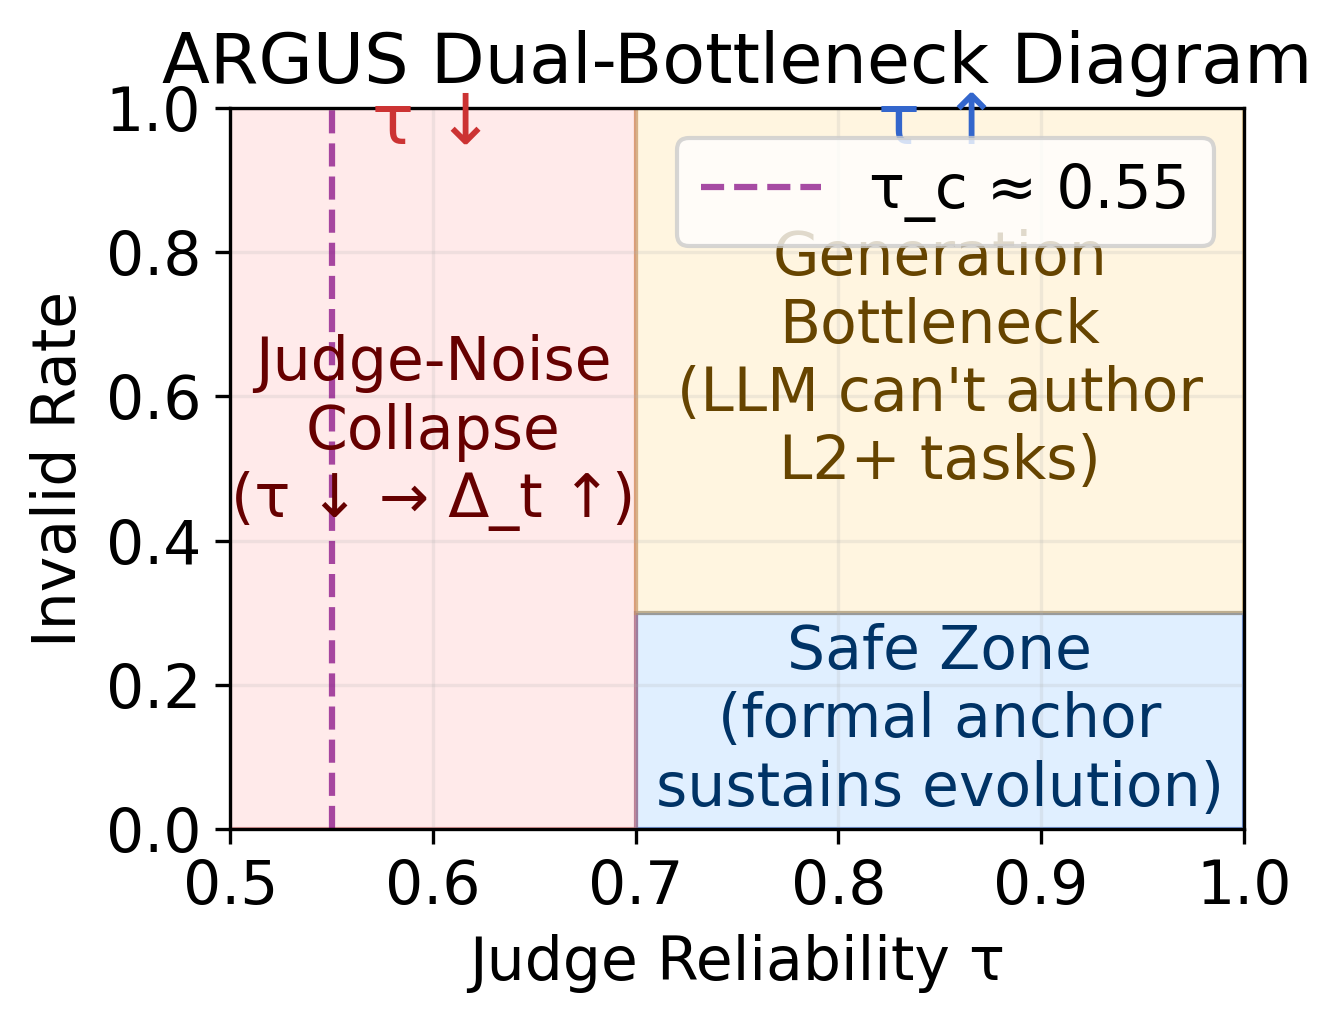
\includegraphics[width=\textwidth]{figures/fig1_dual_bottleneck.png}
  \caption{The safe region is the intersection of two conditions: judge reliability $\tau \ge
  \tau_c$ on the $x$ axis, and generator invalid rate $\le 0.5$ on the $y$ axis. Outside that
  intersection the loop still emits logs and still reports success on the rounds it completes ---
  which is precisely why the failure is easy to miss.}
  \label{fig:dual_bottleneck}
\end{figure*}

\subsection{Judge-Side Bottleneck}

Under the valid-only caliber, condition A (LLM self-score) yields $\Delta_t = 0.150$ while condition
B (Z3 anchor) yields $\Delta_t = 0.000$. The formal anchor therefore eliminates the entire
self-score drift: whenever a task is well-formed, the anchor's verdict \textit{is} the ground truth,
so $\Delta_t$ is identically zero by construction. Under the global caliber the two conditions become
A = 0.243 and B = 0.245, because B's invalid rounds (147 of 600) are charged $\Delta_t = 1.0$. The
apparent contradiction between the two numbers is a caliber difference, not a data inconsistency ---
see Appendix~\ref{app:data_consistency} for the formal definition.

\begin{figure*}[t]
  \centering
  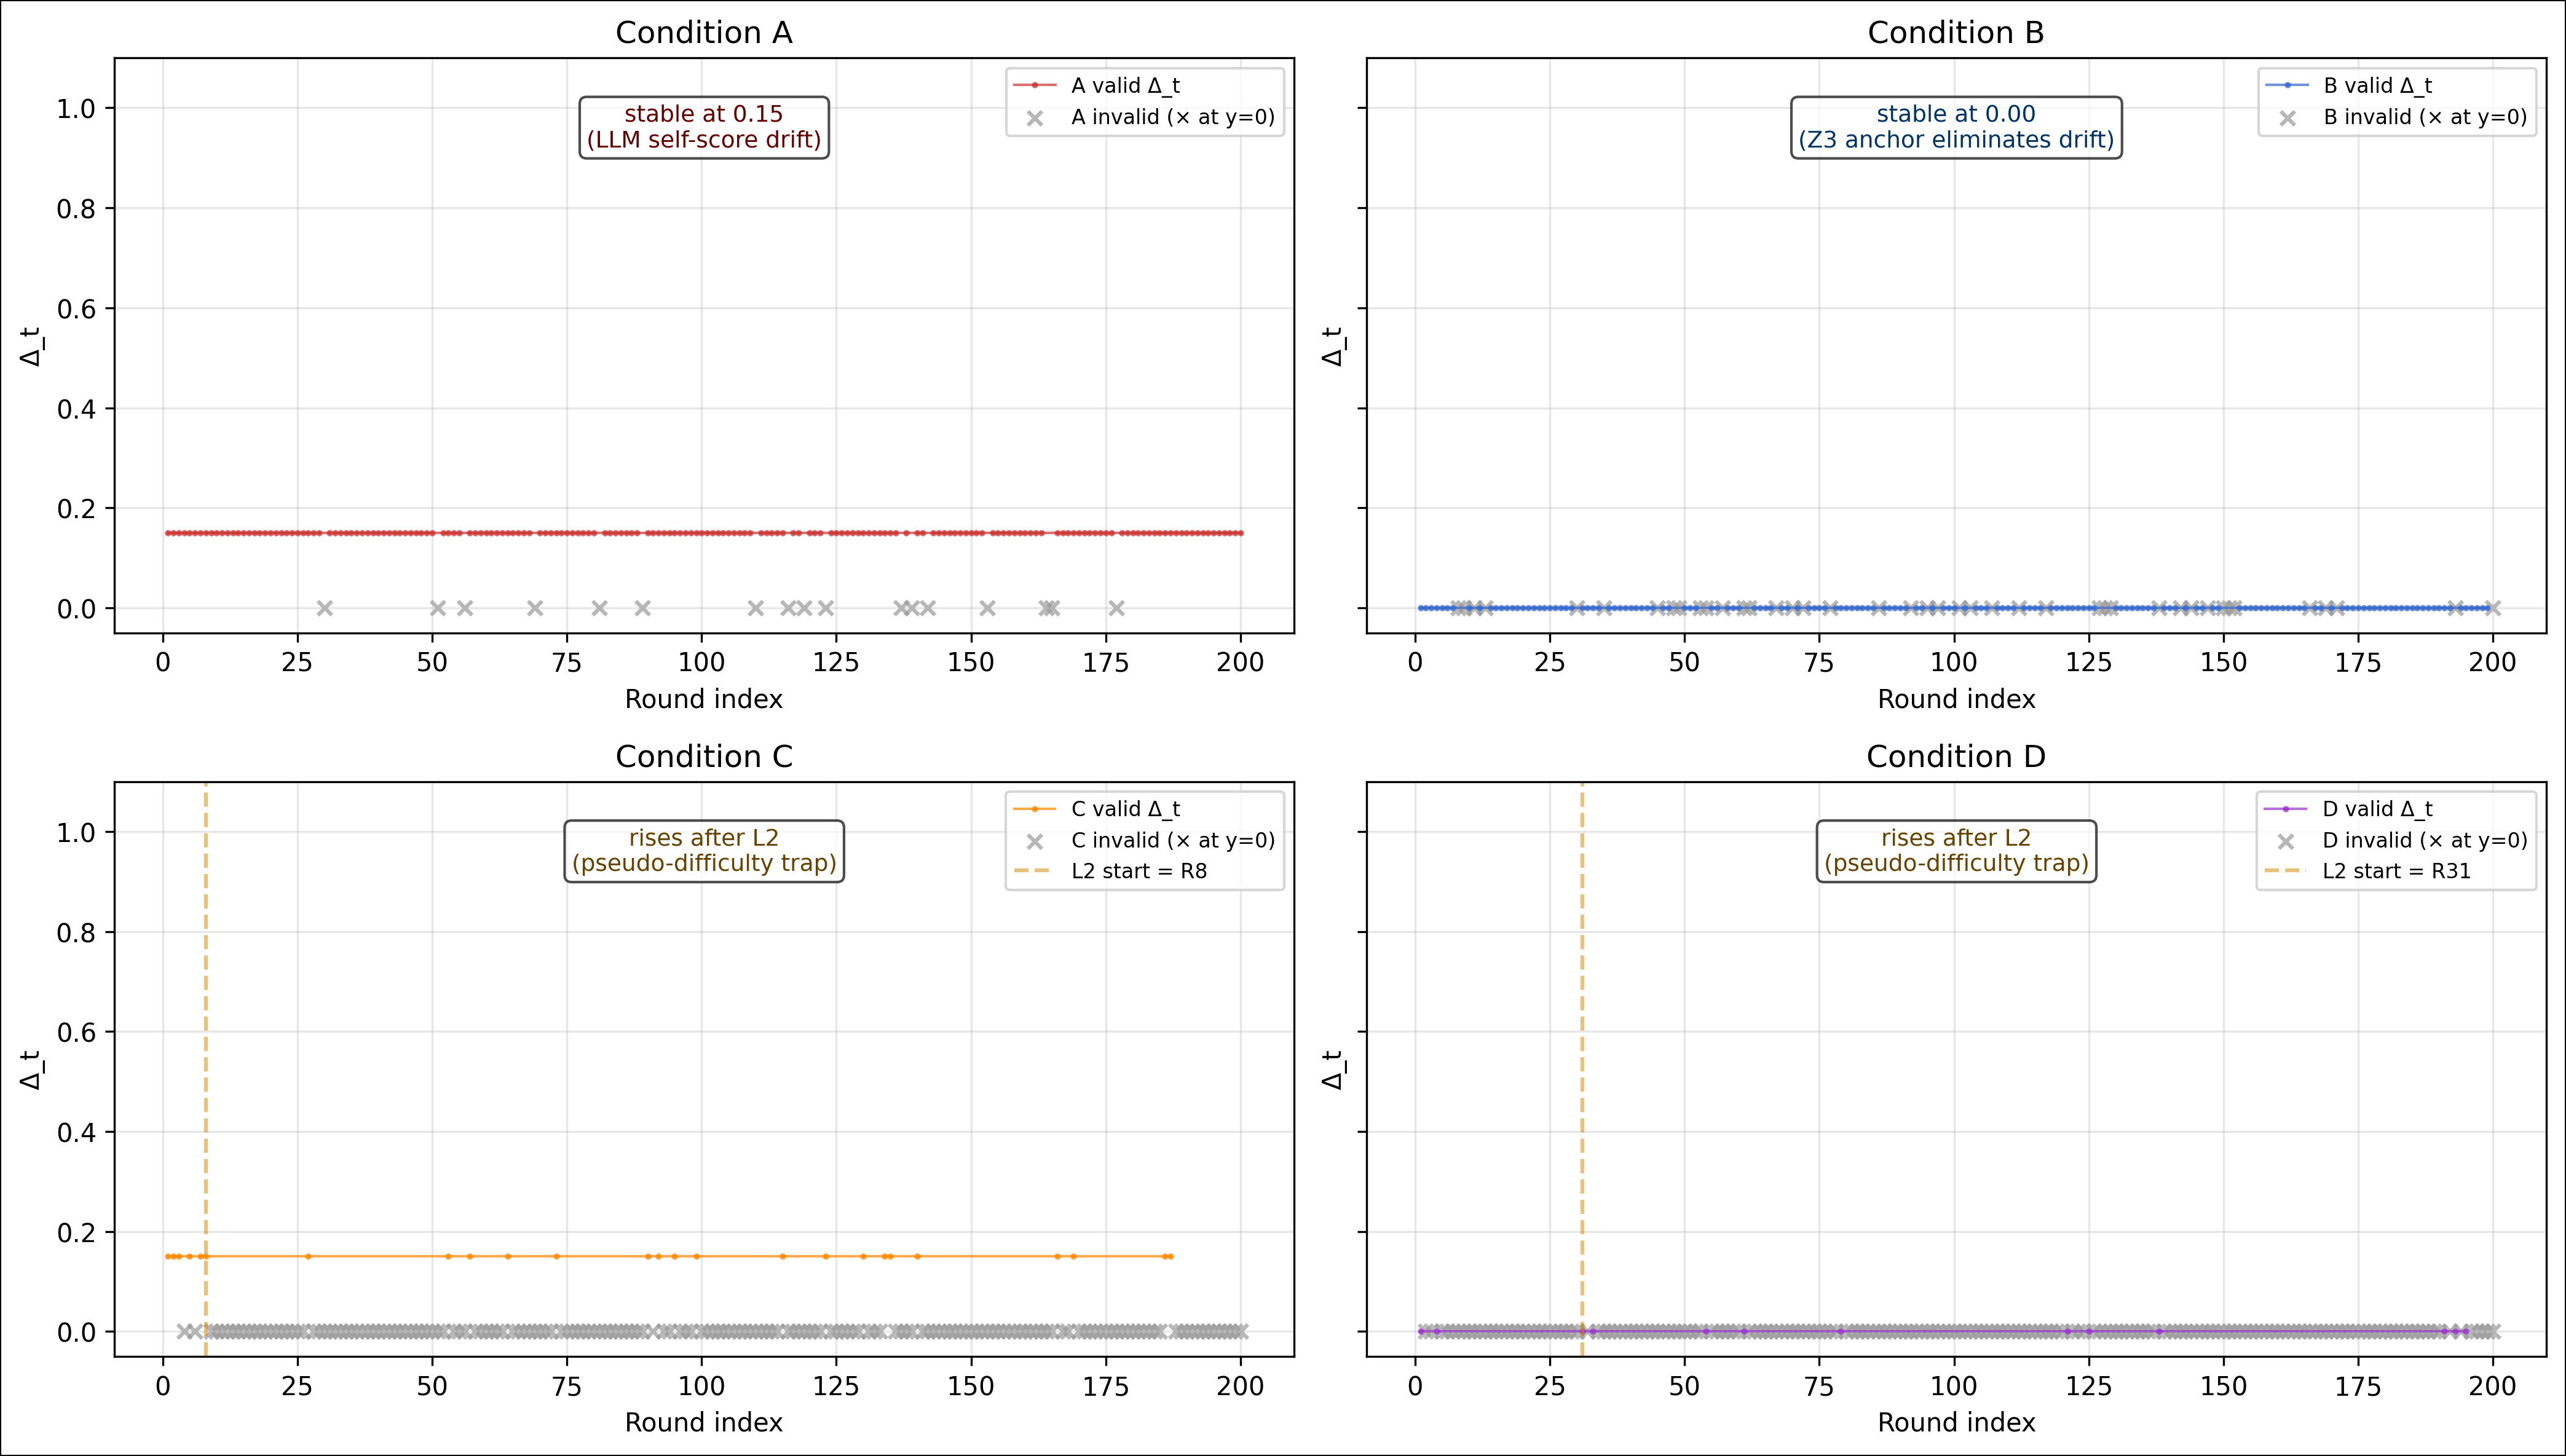
\includegraphics[width=\textwidth]{figures/fig2b_delta_t_per_round.png}
  \caption{Each panel shows one condition; invalid rounds are marked with gray crosses. C/D show the
  pseudo-difficulty trap after L2 transition. Vertical lines mark the first round at which the
  difficulty controller raises the task level.}
  \label{fig:delta_t_per_round}
\end{figure*}

\begin{table}[t]
  \centering
  \caption{Average $\Delta_t$ (valid-only caliber).}
  \label{tab:table2b}
  \small
  \begin{tabularx}{\linewidth}{@{}l*{5}{>{\centering\arraybackslash}X}@{}}
    \toprule
    Condition & $n$ (valid) & Avg $\Delta_t$ (valid only) & Std dev & Min & Max \\
    \midrule
    A & 534 & 0.1500 & 0.0000 & 0.1500 & 0.1500 \\
    B & 453 & 0.0000 & 0.0000 & 0.0000 & 0.0000 \\
    C & 87  & 0.1879 & 0.1394 & 0.1500 & 0.7000 \\
    D & 57  & 0.0000 & 0.0000 & 0.0000 & 0.0000 \\
    \bottomrule
  \end{tabularx}
\end{table}

\subsection{Generator-Side Bottleneck}

Once the population game is enabled (C and D), the difficulty controller pushes tasks toward L2/L3.
The teacher, however, cannot reliably author bit-vector and array constraints: valid rates collapse
from 89.0\% (A) and 75.5\% (B) to 14.5\% (C) and 9.5\% (D). Critically, the failures are \textit{not}
graded by difficulty --- they cluster at the moment of transition, because once the level is raised
the teacher keeps failing and the controller keeps the level high. We call this the
\textbf{pseudo-difficulty trap}: the system believes it is solving harder problems while in fact it
spends its budget on unparseable or unsolvable task proposals.

Importantly, the student is not the bottleneck. Among all 2400 rounds, every round that produced a
valid task was solved correctly; all failures are attributable to task generation.

\begin{figure*}[t]
  \centering
  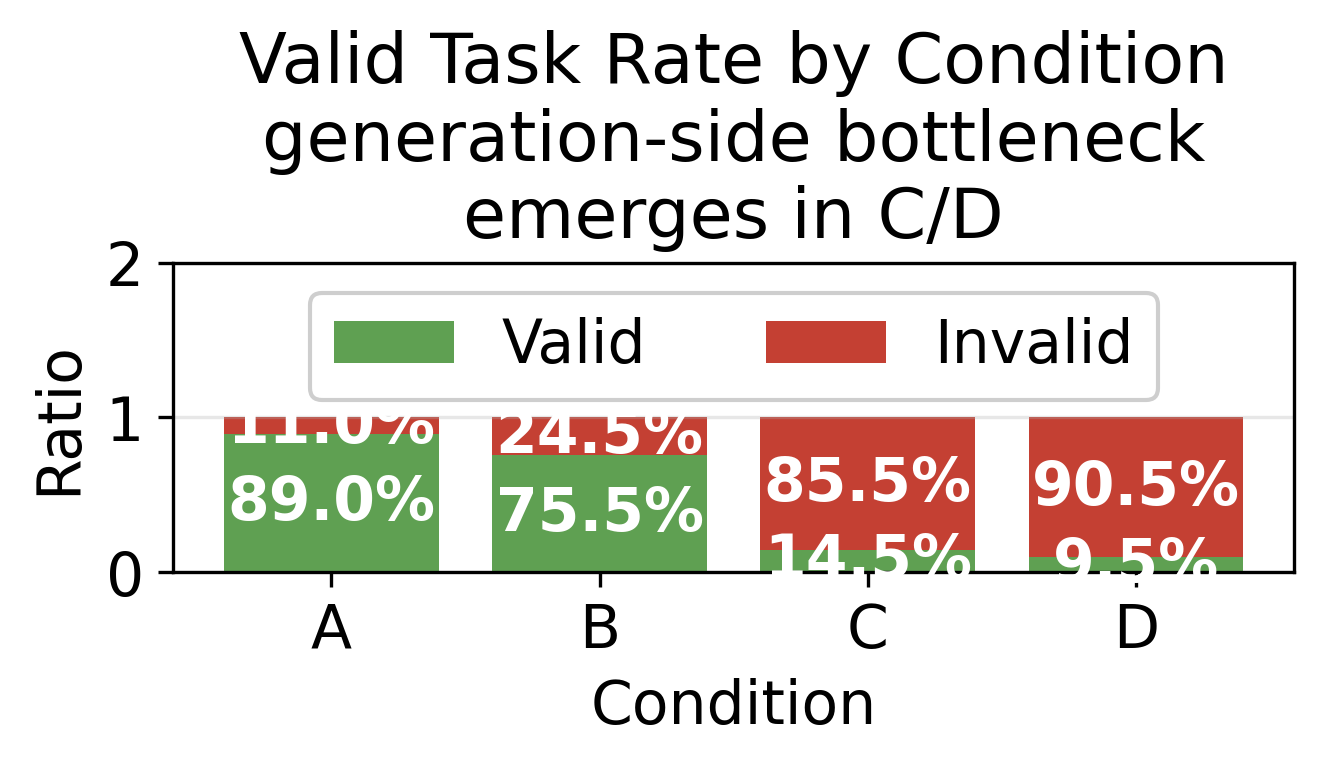
\includegraphics[width=\textwidth]{figures/fig3_validity_rate.png}
  \caption{Overall valid-task rate per condition, collapsing from 89.0\% (A) and 75.5\% (B) to
  14.5\% (C) and 9.5\% (D). B is lower than A not because the anchor performs worse, but because Z3
  anchoring \textit{actively exposes} invalid tasks that A's permissive self-scoring hides.}
  \label{fig:validity_by_condition}
\end{figure*}

\begin{table}[t]
  \centering
  \caption{Valid task rate by condition.}
  \label{tab:table3}
  \small
  \begin{tabularx}{\linewidth}{@{}l*{4}{>{\centering\arraybackslash}X}@{}}
    \toprule
    Condition & Valid & Invalid & Valid rate & Correct rate (valid subset) \\
    \midrule
    A & 534 & 66  & 0.8900 & 1.0000 \\
    B & 453 & 147 & 0.7550 & 1.0000 \\
    C & 87  & 513 & 0.1450 & 1.0000 \\
    D & 57  & 543 & 0.0950 & 1.0000 \\
    \bottomrule
  \end{tabularx}
\end{table}

\subsection{Budget Decomposition}

The two bottlenecks therefore \textbf{share one budget}. Given a tolerated global error
$\Delta_t^{\max}$, the amount left for judge noise is

\[
  \Delta_{\text{judge}}^{\text{budget}} = 1 - \frac{1-\Delta_t^{\max}}{1-\Delta_t^{\text{gen}}}
  \qquad\Longrightarrow\qquad
  \tau_c = \sqrt{1 - 2\,\Delta_{\text{judge}}^{\text{budget}}}
\]

$\tau_c$ is thus not an intrinsic property of a condition's mechanisms --- it is \textbf{derived}
from how much of the budget the generator bottleneck leaves over. A condition with a large
$\Delta_t^{\text{gen}}$ needs a more reliable judge for the same overall tolerance, but the driver is
the budget split, not $\tau_c$ itself.

Concretely, at $\Delta_t^{\max} = 0.60$: condition B ($\Delta_t^{\text{gen}} = 0.245$) requires
$\tau_c \approx 0.24$, while C and D ($\Delta_t^{\text{gen}} = 0.855$ and $0.905$) cannot meet the
budget at \textbf{any} judge reliability, because their generator bottleneck alone already exceeds
it. That is the correct form of the Q4 intuition, and it turns the dual-bottleneck framework from a
diagnosis into an accounting rule.

\begin{table}[t]
  \centering
  \caption{Budget decomposition: the judge budget left over once the generator
  bottleneck is accounted for, and the judge reliability it requires.}
  \label{tab:table4cbudget}
  \small
  \begin{tabularx}{\linewidth}{@{}l*{4}{>{\centering\arraybackslash}X}@{}}
    \toprule
    Condition & $\Delta_t^{\text{gen}}$ & $\Delta_t^{\max}$ & judge budget
    & required $\tau_c$ \\
    \midrule
    A & 0.1100 & 0.60 & $0.5506$ & $\ge 0$ (random suffices) \\
    B & 0.2450 & 0.60 & $0.4702$ & 0.244 \\
    C & 0.8550 & 0.60 & $-1.7586$ & unreachable \\
    D & 0.9050 & 0.60 & $-3.2105$ & unreachable \\
    \midrule
    A & 0.1100 & 0.70 & $0.6629$ & $\ge 0$ (random suffices) \\
    B & 0.2450 & 0.70 & $0.6026$ & $\ge 0$ (random suffices) \\
    C & 0.8550 & 0.70 & $-1.0690$ & unreachable \\
    D & 0.9050 & 0.70 & $-2.1579$ & unreachable \\
    \midrule
    A & 0.1100 & 0.80 & $0.7753$ & $\ge 0$ (random suffices) \\
    B & 0.2450 & 0.80 & $0.7351$ & $\ge 0$ (random suffices) \\
    C & 0.8550 & 0.80 & $-0.3793$ & unreachable \\
    D & 0.9050 & 0.80 & $-1.1053$ & unreachable \\
    \bottomrule
  \end{tabularx}
\end{table}

% ===========================================================================
% 5. JUDGE RELIABILITY THRESHOLD
% ===========================================================================
\section{Judge Reliability Threshold}

\subsection{Noise Injection Protocol}

We model an unreliable judge by flipping its verdict with probability $(1 - \tau)/2$, where
$\tau \in [0, 1]$ is the judge reliability. The flip is applied symmetrically (SAT $\to$ UNSAT and
UNSAT $\to$ SAT); error and unknown verdicts are never flipped, since they carry no truth value to
invert. Each $(\tau, \text{condition})$ cell uses a fixed noise seed so the experiment is
bit-for-bit reproducible. The protocol is implemented in
\texttt{argus/z3\_anchor.py::verify\_with\_noise}.

A detail that matters for Section~5.3: in this configuration \textbf{two independent judgments} are
noised per round --- the teacher's verdict on the generated task, and the student's verdict on its
own encoding. They are produced by separate Z3 calls and therefore flip independently.

\subsection{Empirical $\tau_c$}

We sweep $\tau$ over eight values $\{0.55, 0.60, 0.65, 0.70, 0.75, 0.80, 0.90, 1.00\}$ for
conditions B and D, with 50 rounds per cell (800 rounds total) using the \textbf{real} DeepSeek V4
Flash API. All rounds are pinned to difficulty L1 so that the generator-side bottleneck is held
constant and only the judge's reliability varies.

The original hypothesis was that $\tau_c(D) > \tau_c(B)$ because D's population game advances the
difficulty into L2/L3. Under L1 isolation the real-API sweep returns
\textbf{$\tau_c(D) = \tau_c(B) = 0.55$}, and an earlier mock-LLM gap of 0.90 vs 0.55 does not
reproduce. Pinning the difficulty removes exactly the mechanism the hypothesis invoked; the mock gap
was an artefact of deterministic task content collapsing $\Delta_t$ to a $\{0, 1\}$ sequence. The
hypothesis as stated is \textbf{not supported}.

Across the eight swept $\tau$ values the measured per-cell mean $\Delta_t$ falls monotonically from
0.30 at $\tau = 0.55$ to 0.00 at $\tau = 1.00$ for condition B. The shape is a parabola opening
downward, not a straight line, and it passes through 0.5 at $\tau = 0$ rather than through 1.0. Both
features turn out to be diagnostic of the mechanism, as Section~5.3 shows.

\begin{figure}[t]
  \centering
  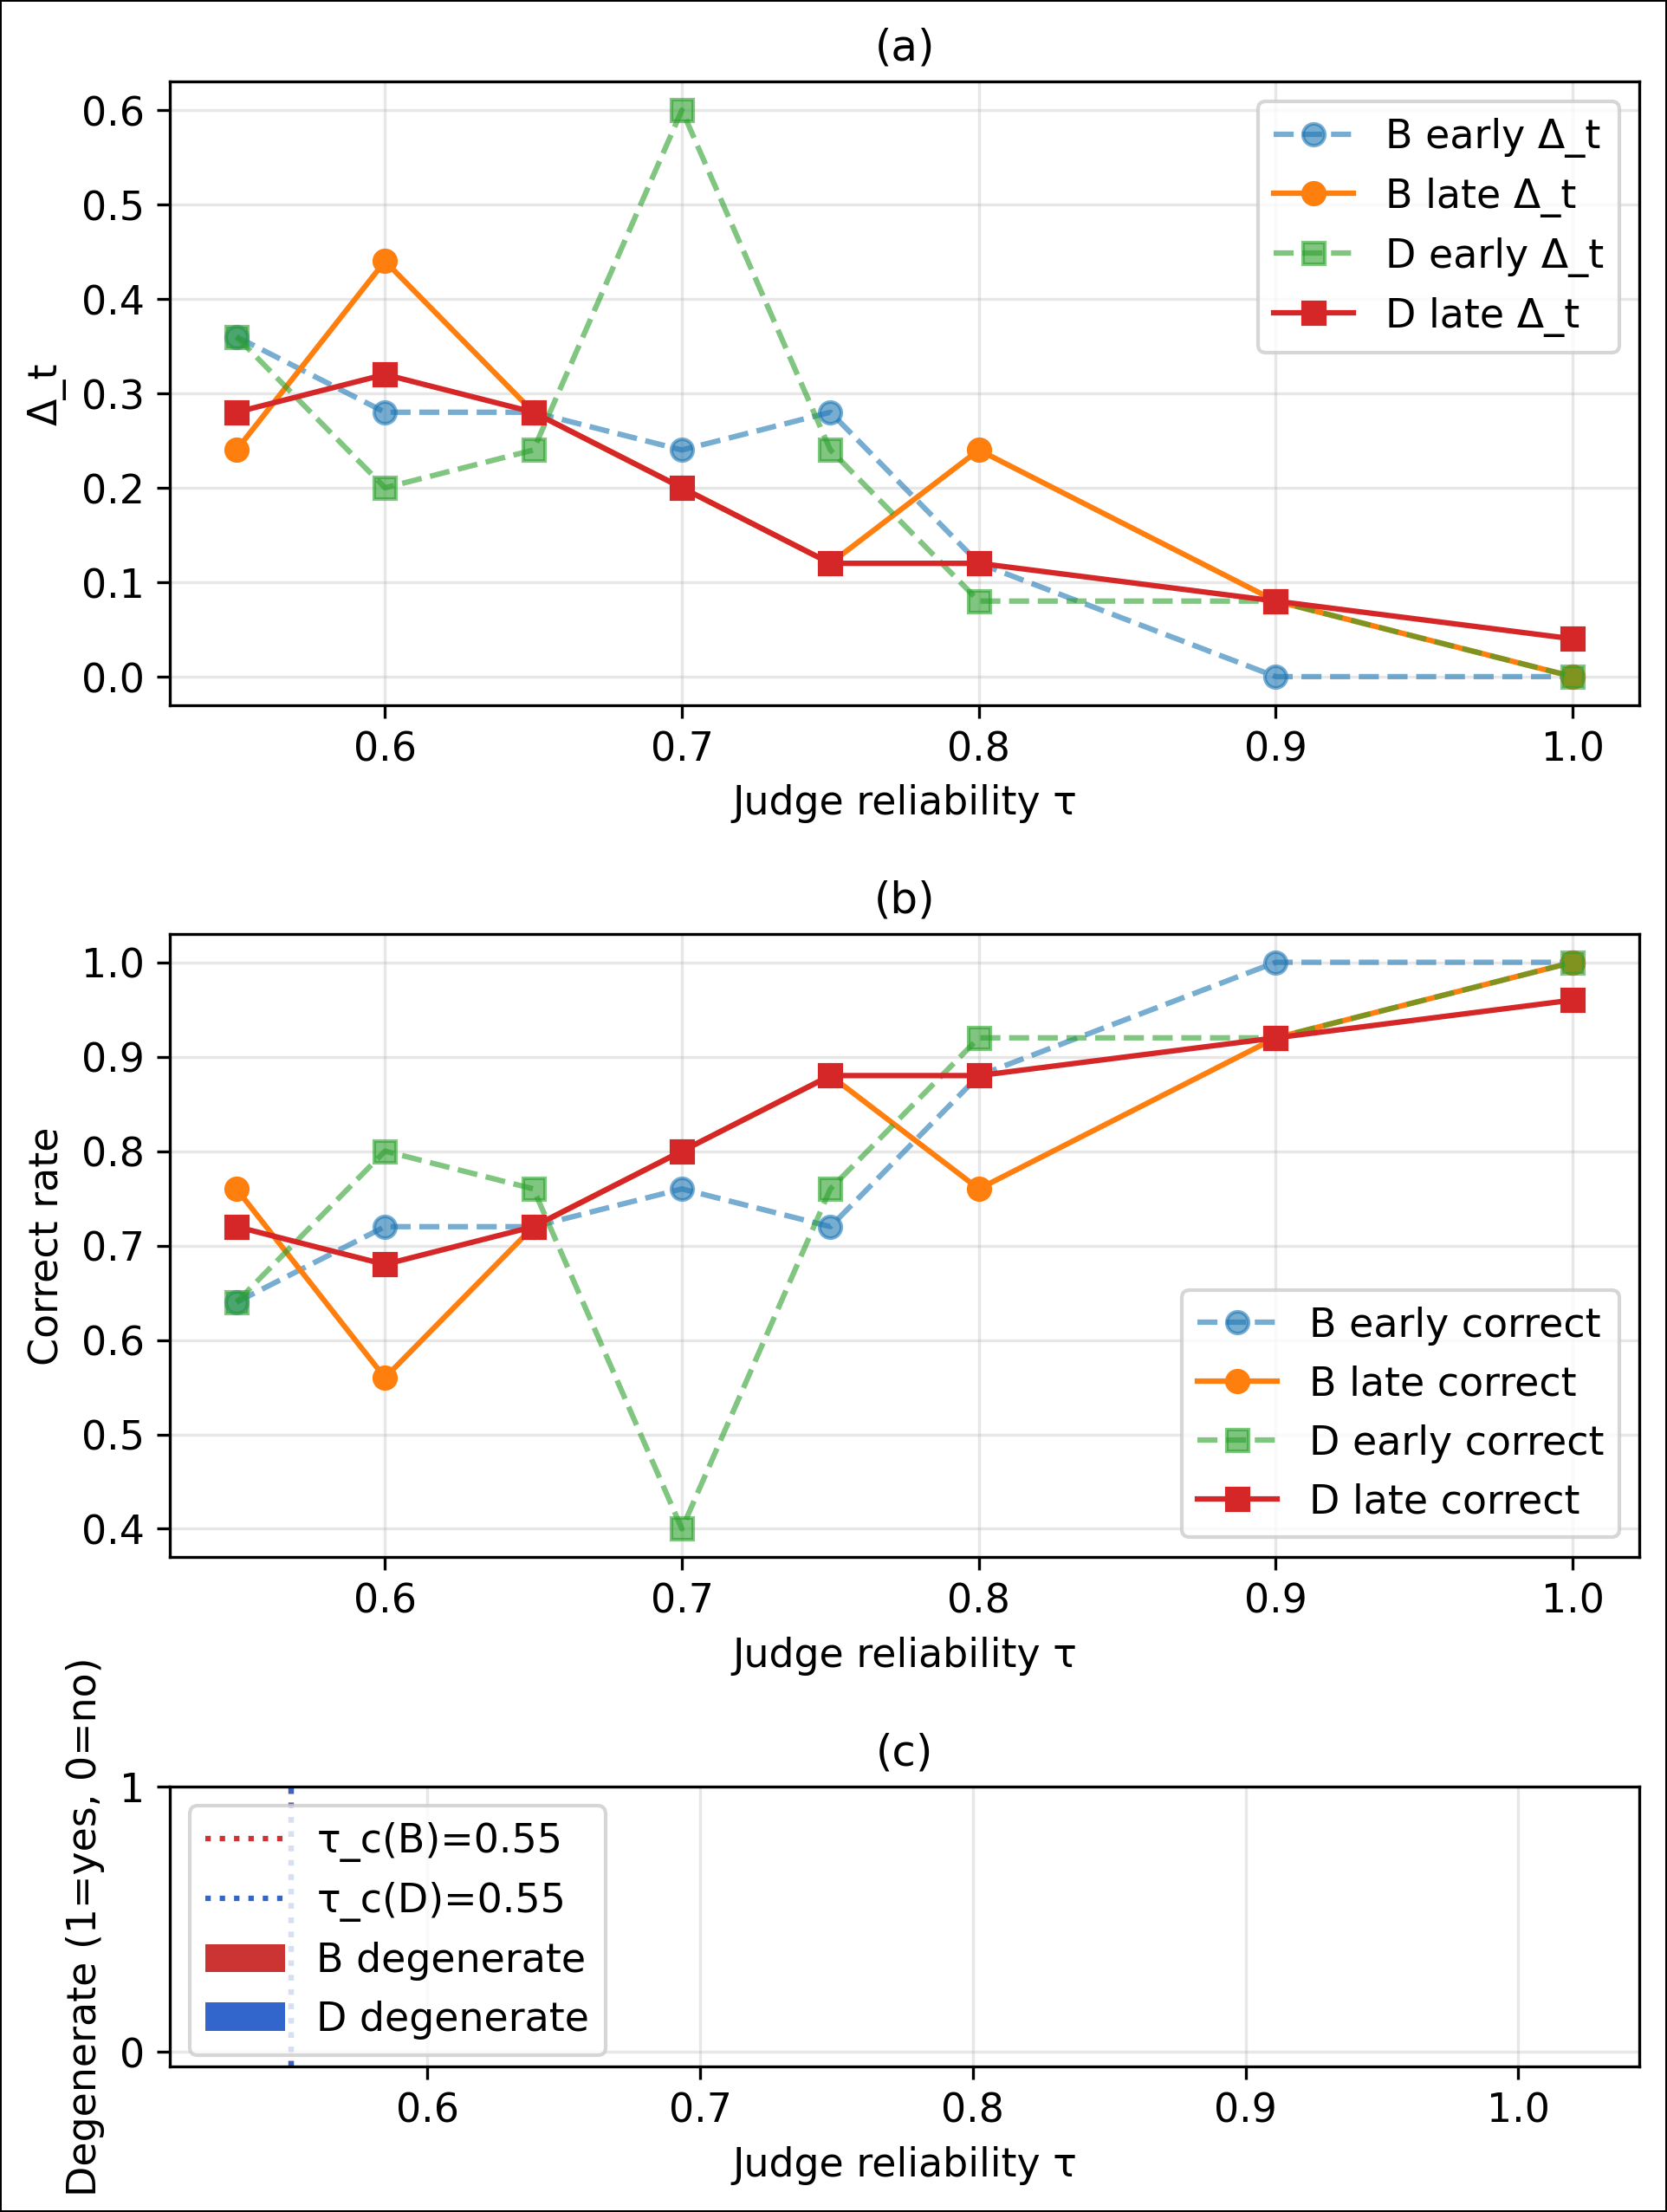
\includegraphics[width=\columnwidth]{figures/fig5_tau_c_curve_real.png}
  \caption{The $\tau$-gradient sweep on the real API: 8 $\tau$ values $\times$ 2 conditions (B/D)
  $\times$ 50 rounds = 800 rounds. Under the within-$\tau$ degeneration criterion no $\tau$ value
  degenerates, so the reported $\tau_c = 0.55$ is the lower edge of the swept grid and should be
  read as an upper bound, not as the system's tolerance. Panel (c) is empty because no $\tau$ value
  degenerates under the within-$\tau$ criterion; the two vertical lines mark
  $\tau_c(B) = \tau_c(D) = 0.55$.}
  \label{fig:tau_c_curve}
\end{figure}

\begin{table}[t]
  \centering
  \caption{Judge reliability threshold $\tau_c$ (real API).}
  \label{tab:table4}
  \small
  \begin{tabularx}{\linewidth}{@{}l*{4}{>{\centering\arraybackslash}X}@{}}
    \toprule
    Condition & $\tau_c$ (combined) & $\tau_c$ ($\Delta_t$ caliber) & $\tau_c$ (correct-rate caliber) & Degenerate $\tau$ values \\
    \midrule
    Condition B & 0.55 & 0.55 & 0.55 & (none) \\
    Condition D & 0.55 & 0.55 & 0.55 & (none) \\
    \bottomrule
  \end{tabularx}
\end{table}

\subsection{Analytical Formula}

\textbf{Assumption 1 (judge noise).} Each Z3 verdict is independently flipped with probability

\[
  p = \frac{1-\tau}{2}
\]

\textbf{Assumption 2 (two independent judgments per round).} A round involves two separate Z3 calls:
one validating the task the teacher produced (which becomes \texttt{expected}), and one validating
the answer the student submitted. They are separate processes and flip independently.

A round is scored correct exactly when the two verdicts \textbf{agree} --- both unflipped, or both
flipped:

\[
  P(\text{correct}) = (1-p)^2 + p^2
\]

Substituting $p = (1-\tau)/2$, so that $1-p = (1+\tau)/2$:

\[
  P(\text{correct}) = \left(\frac{1+\tau}{2}\right)^2 + \left(\frac{1-\tau}{2}\right)^2
  = \frac{(1+\tau)^2 + (1-\tau)^2}{4} = \frac{2 + 2\tau^2}{4} = \frac{1+\tau^2}{2}
\]

and therefore

\[
  \boxed{\;\Delta_t(\tau) = 1 - P(\text{correct}) = \frac{1-\tau^2}{2}\;}
\]

\textbf{Where the $\tau^2$ comes from.} It is the sum of the two agreement terms: both-correct
contributes $((1+\tau)/2)^2$ and both-flipped contributes $((1-\tau)/2)^2$. The cross terms cancel,
leaving $(1+\tau^2)/2$. The exponent 2 is therefore the number of independent judgments per round
--- not any property of the judge alone.

\textbf{Where the $1/2$ comes from.} At $\tau = 0$ the expression gives $\Delta_t = 1/2$: two
independent random verdicts agree half the time. This is the binary symmetry of SAT/UNSAT tasks, and
it is why the curve is anchored at 0.5 rather than 1.0 on the left.

Across the eight swept $\tau$ values the measured per-cell means track the closed form with

\begin{itemize}
  \item MAE = \textbf{0.0258}, RMSE = 0.0329 (condition B)
  \item MAE = \textbf{0.0520}, RMSE = 0.0660 (condition D)
\end{itemize}

\textbf{A discriminating test.} The mechanism in Assumption 2 is not the only story that yields the
same $\Delta_t(\tau)$. An alternative --- that the judge judges correctly with probability $\tau$
\textit{and} the system accepts that judgment with probability $\tau$ --- predicts
$P(\text{correct}) = \tau^2$ instead of $(1+\tau^2)/2$. These two differ sharply, so the measured
\texttt{correct\_rate} separates them without any fitting:

\begin{center}
\small
\begin{tabular}{@{}llr@{}}
  \toprule
  Model & $P(\text{correct})$ & MAE vs observed \texttt{correct\_rate} \\
  \midrule
  Two independent judgments (\textbf{this work}) & $(1 + \tau^2)/2$ & \textbf{0.0389} \\
  Judge + acceptance & $\tau^2$ & 0.2291 \\
  \bottomrule
\end{tabular}
\end{center}

Over the 16 $(\tau, \text{condition})$ cells the two-judgment model is closer in 13, tied in 2, and
loses in 1. At $\tau = 0.80$ / condition B it predicts 0.8200 against a measured 0.8200. The
acceptance story is rejected by a factor of six in MAE.

\textbf{Inverting the model.} Solving $\Delta_t = (1 - \tau^2)/2$ for $\tau$ gives the design rule

\[
  \tau_c = \sqrt{1 - 2\,\Delta_t^{\max}}
\]

so a system that can tolerate an error floor of $\Delta_t^{\max}$ requires a judge of at least that
reliability:

\begin{center}
\small
\begin{tabular}{@{}rr@{}}
  \toprule
  $\Delta_t$ budget & Required $\tau_c$ \\
  \midrule
  0.05 & 0.949 \\
  0.10 & 0.894 \\
  0.15 & 0.837 \\
  0.20 & 0.775 \\
  0.25 & 0.707 \\
  \bottomrule
\end{tabular}
\end{center}

This is the practically useful form of the result: it converts a tolerance on evaluation error into
a minimum reliability requirement for the judge, without needing to re-run the sweep. Note the
reachability bound --- no judge reliability can hold $\Delta_t$ below 0.5, since $\Delta_t(0) = 1/2$.

\begin{figure}[t]
  \centering
  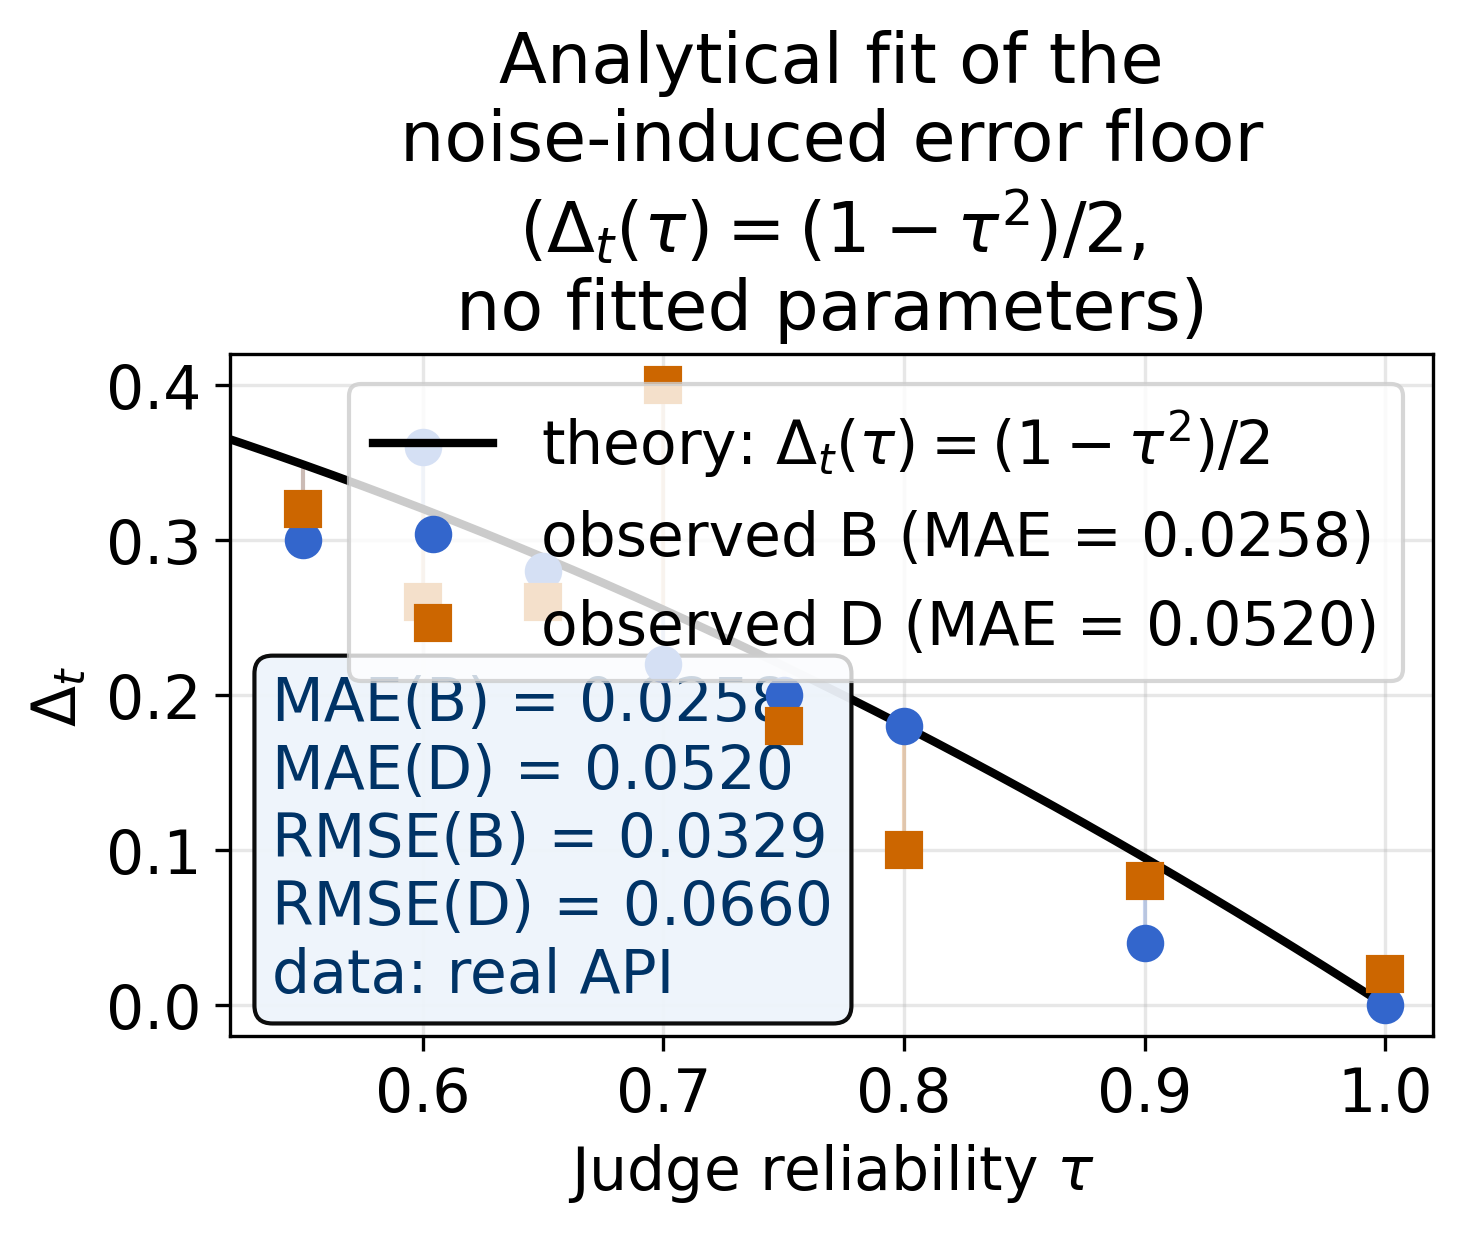
\includegraphics[width=\columnwidth]{figures/fig5b_tau_c_analytical.png}
  \caption{The closed form $\Delta_t(\tau) = (1 - \tau^2)/2$ against the observed scatter. The
  formula has no free parameters; measured MAE over 50 rounds per $\tau$ cell is 0.0258 (B) and
  0.0520 (D). The curve is anchored at 0.5 rather than 1.0 when $\tau = 0$, which is the binary
  symmetry of two independent verdicts.}
  \label{fig:analytical_fit}
\end{figure}

\subsection{Theorem 1: Judge Reliability Threshold}

Under the assumptions stated in Section~5.3, we state the threshold as a theorem.

\textbf{Theorem 1.} \textit{The expected evaluation bias of the system is}

\[
  \Delta_t(\tau) \;=\; \frac{1-\tau^{2}}{2}
\]

\textit{with no free parameters; equivalently $P(\text{correct}) = (1+\tau^{2})/2$, and
$\Delta_t(0) = 1/2$.}

\textbf{Inverse (design) form.} Solving for $\tau$ gives the minimum admissible judge reliability at
a tolerated bias $\Delta_t^{\max}$:

\[
  \tau_c \;=\; \sqrt{1 - 2\,\Delta_t^{\max}}
\]

Because $\Delta_t(0) = 1/2$, no judge reliability can hold the bias below $1/2$, so the rule is
defined only for $\Delta_t^{\max} \in [0, 1/2)$.

\textbf{Corollary (judge scarcity).} $\tau_c$ is a function of the tolerated bias, \textbf{not} a
constant of the system. At $\Delta_t^{\max} = 0.35$ a judge that errs on roughly one verdict in five
($\tau \approx 0.55$) still keeps the system inside the safe region; tightening the tolerance to
$0.05$ requires $\tau \approx 0.95$.

\textbf{Empirical validation.} Fitted against 800 real-API rounds (8 $\tau$ values $\times$ 2
conditions $\times$ 50 rounds, difficulty pinned to L1): MAE = \textbf{0.0258} / RMSE = 0.0329 (B)
and MAE = \textbf{0.0520} / RMSE = 0.0660 (D).

\textbf{Remark (rejected alternative model).} A competing model --- the judge is correct with
probability $\tau$ \textit{and} the system accepts that judgment with probability $\tau$ --- predicts
$P(\text{correct}) = \tau^{2}$, hence $\Delta_t = 1-\tau^{2}$. It is rejected \textbf{without any
fitting} by the discriminating test: MAE 0.2291 against the observed \texttt{correct\_rate}, versus
0.0389 for Theorem 1, with Theorem 1 closer in 13 of the 16 cells, tied in 2 and losing in 1. At
$\tau = 0.55$ it predicts 0.6975 against a measured 0.3000 (B) and 0.3200 (D). No result in this
paper uses $\Delta_t = 1-\tau^{2}$.

\textbf{Empirical $\tau_c$.} Under L1 isolation no $\tau$ triggers the within-$\tau$ degeneration
criterion, so the detected value is $\tau_c(B) = \tau_c(D) =$ \textbf{0.55} --- the lower edge of the
swept grid, to be read as an \textbf{upper bound} rather than the system's true tolerance. The closed
form maps it to $\Delta_t^{\max} = (1-0.55^{2})/2 = 0.34875 \approx$ \textbf{0.349}, consistent with
the measured per-cell bias at that $\tau$ (0.300 B / 0.320 D) to within the fit's MAE.

\textbf{Relation to the Ratchet bound.} Ratchet's analysis gives $(1 - \tau)/2$ as the probability
that a \textbf{single} judgment is flipped. Our quantity is the steady-state error of a
\textbf{double}-judgment system. The two are related by the agreement probability, and the
distinction is structural rather than numerical:

\begin{center}
\small
\begin{tabular}{@{}lll@{}}
  \toprule
  Setting & Noisy events per decision & Error \\
  \midrule
  Skill elimination (Ratchet) & one judgment, then act on it & $(1 - \tau)/2$ \\
  Answer evaluation (this work) & judge's verdict \textbf{and} system's verdict must agree & $(1 - \tau^2)/2$ \\
  \bottomrule
\end{tabular}
\end{center}

The map between them is the probability that exactly one of the two judgments flips:

\[
  \Delta_t = 2p(1-p) \;\xrightarrow{p \to 0}\; 2p = 1-\tau
\]

So the two agree to first order in the high-reliability limit, and diverge quadratically away from
it. At $\tau = 0.95$ the single-judgment bound predicts 0.025 while the double-judgment model
predicts 0.049: requiring two independent verdicts to agree costs a factor of two in tolerated error
at that reliability. Ratchet's bound is the special case of a system that acts on one judgment; the
formula here generalises it to systems that act on agreement between two.

\begin{figure*}[t]
  \centering
  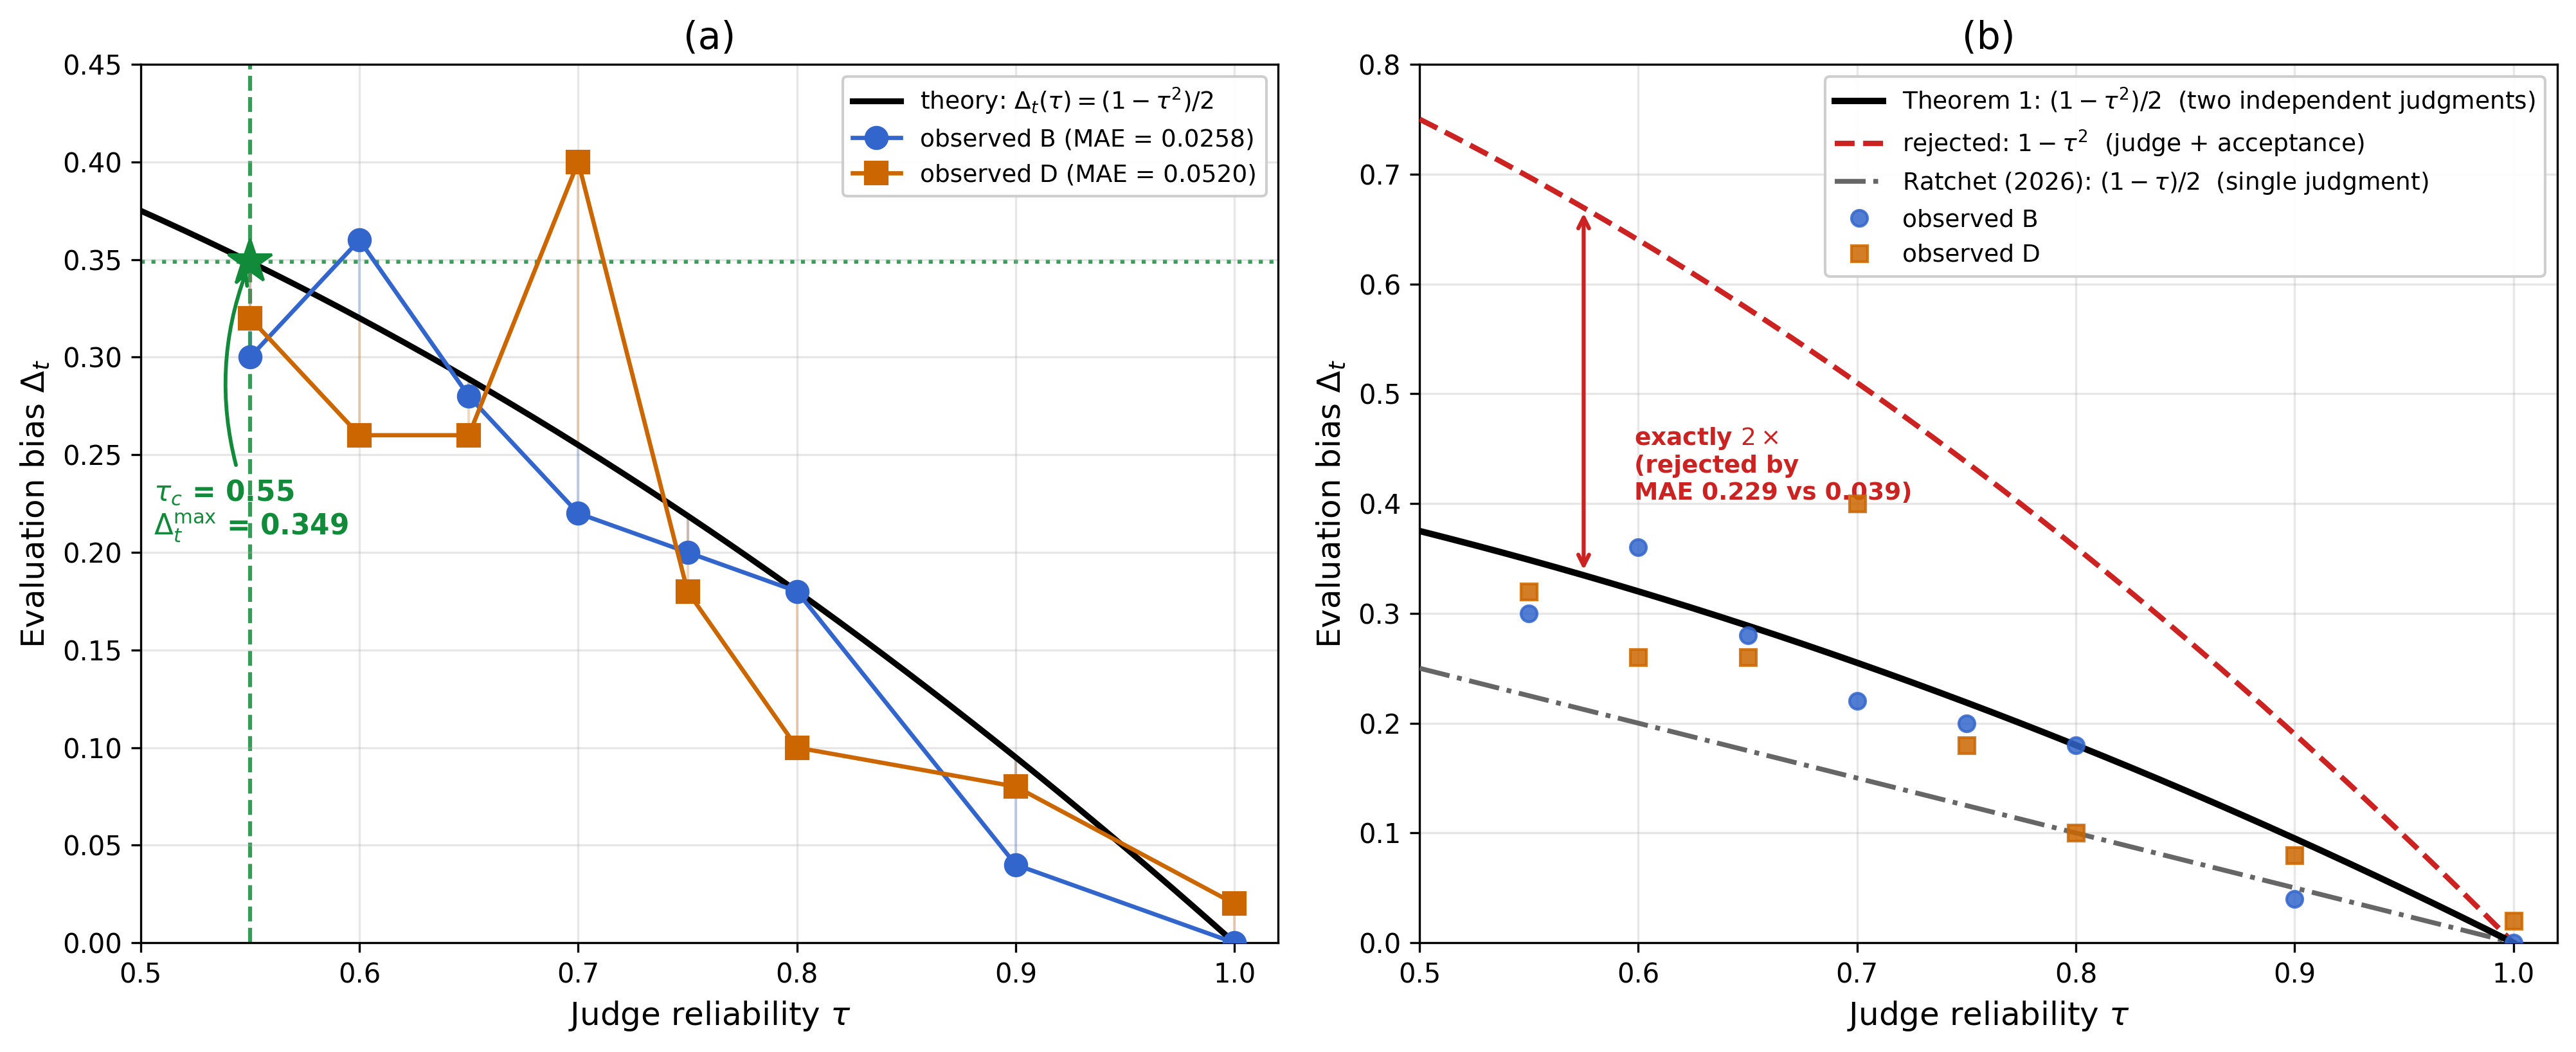
\includegraphics[width=\textwidth]{figures/fig5c_theorem1.png}
  \caption{Panel (a): the closed form $\Delta_t(\tau) = (1-\tau^2)/2$ against the real-API sweep for
  conditions B and D, with the measured $\tau_c = 0.55$ and the corresponding
  $\Delta_t^{\max} = 0.349$ marked. Panel (b): the same closed form against the rejected acceptance
  model ($\Delta_t = 1-\tau^2$) and Ratchet's single-judgment bound ($(1-\tau)/2$); the acceptance
  model runs exactly twice as high and is rejected by the discriminating test of Section~5.3.}
  \label{fig:theorem1}
\end{figure*}

% ===========================================================================
% 6. EXTENDING GENERATOR CAPABILITY
% ===========================================================================
\section{Extending Generator Capability}

\subsection{Four-Layer Constraint Framework}

Section~4.3 showed that free-form code generation is the binding constraint on the generator side. We
therefore replace it with a four-layer pipeline:

\begin{enumerate}
  \item \textbf{JSON skeleton generation.} The teacher prompt asks for a JSON object
        (\texttt{variables}, \texttt{constraints}, \texttt{expected\_sat}) instead of Python code,
        removing the bracket-matching and variable-declaration failure classes outright.
  \item \textbf{Deterministic rendering.} \texttt{render\_z3\_code} turns the skeleton into Z3 Python
        code by template substitution. Because the renderer never guesses, the output is
        syntactically valid by construction; malformed skeletons raise a typed
        \texttt{TaskJSONInvalid} rather than failing silently.
  \item \textbf{Symbolic feedback.} Z3 error codes are mapped to symbolic constraints (for example, a
        timeout appends ``reduce the constraint count to at most five'') which are injected into the
        next attempt's prompt.
  \item \textbf{Curriculum controller.} Sub-level variable counts within each difficulty level are
        raised after five consecutive rounds with valid rate $> 0.80$ and lowered after three
        consecutive rounds below $0.50$, damping the oscillation that produced the pseudo-difficulty
        trap.
\end{enumerate}

\subsection{Real API Validation}

We validate the constraint framework on 240 rounds (4 conditions $\times$ 3 levels $\times$ 20
rounds) using real DeepSeek V4 Flash API. This is a capability probe rather than a full replication
of the 2400-round baseline: the legacy comparison uses the existing 2400-round logs, while the
framework is measured on a deliberately smaller budget because each level is requested explicitly
rather than left to the difficulty controller.

With the framework in place, valid rates under the real API are L1 = 98.8\% (79/80), L2 = 71.2\%
(57/80), L3 = 58.8\% (47/80). The legacy teacher, by contrast, produced only a handful of L2/L3 valid
tasks across 2400 rounds (11 and 114 respectively), because most attempts failed before a task could
be verified at all. Because the two runs use different round budgets and different denominators, this
compares \textbf{capability}, not rates.

The first real-API run of the framework scored 100\% on L1 but only 10\% on L2. Every failure carried
the same diagnostic: the validator tokenised constraints with a bare identifier regex, which splits
the hexadecimal literal \texttt{0x0F} into \texttt{0} and \texttt{x0F}; the fragment was then
rejected as an undeclared variable. L1 (integer arithmetic) rarely uses hex masks, so it was
unaffected; L2 is bit-vector theory, where \texttt{0xFF}-style masks are the standard idiom, so the
validator rejected essentially every well-formed task. The failure was in our own guardrail, not in
the model.

The fix substitutes numeric literals (hex, binary, octal, decimal, underscore-separated, scientific)
with placeholders before scanning, and extends the Z3 builtin whitelist (\texttt{BitVecVal},
\texttt{BV2Int}, \texttt{LShR}, \ldots). L2 rose from 10\% to 71.2\% and L3 reached 58.8\%. Seven
regression tests pin the behaviour.

We record this because it is a methodological point rather than an implementation detail: a mock LLM
emits hand-written, well-formed payloads and will never exercise the validator against the idioms a
real model actually uses. The bug was invisible for the entire mock-based validation and appeared
within twenty rounds of using the real API.

After the fix, the remaining invalid rounds are all
\texttt{error\_code=1: LLM did not return valid JSON} --- the model produced output that could not be
parsed at all. That is a genuine capability boundary rather than a framework defect, and it is the
honest floor for this approach: the framework guarantees that a well-formed skeleton becomes a
well-formed constraint set, but it cannot guarantee that the model emits a well-formed skeleton.

\begin{figure*}[t]
  \centering
  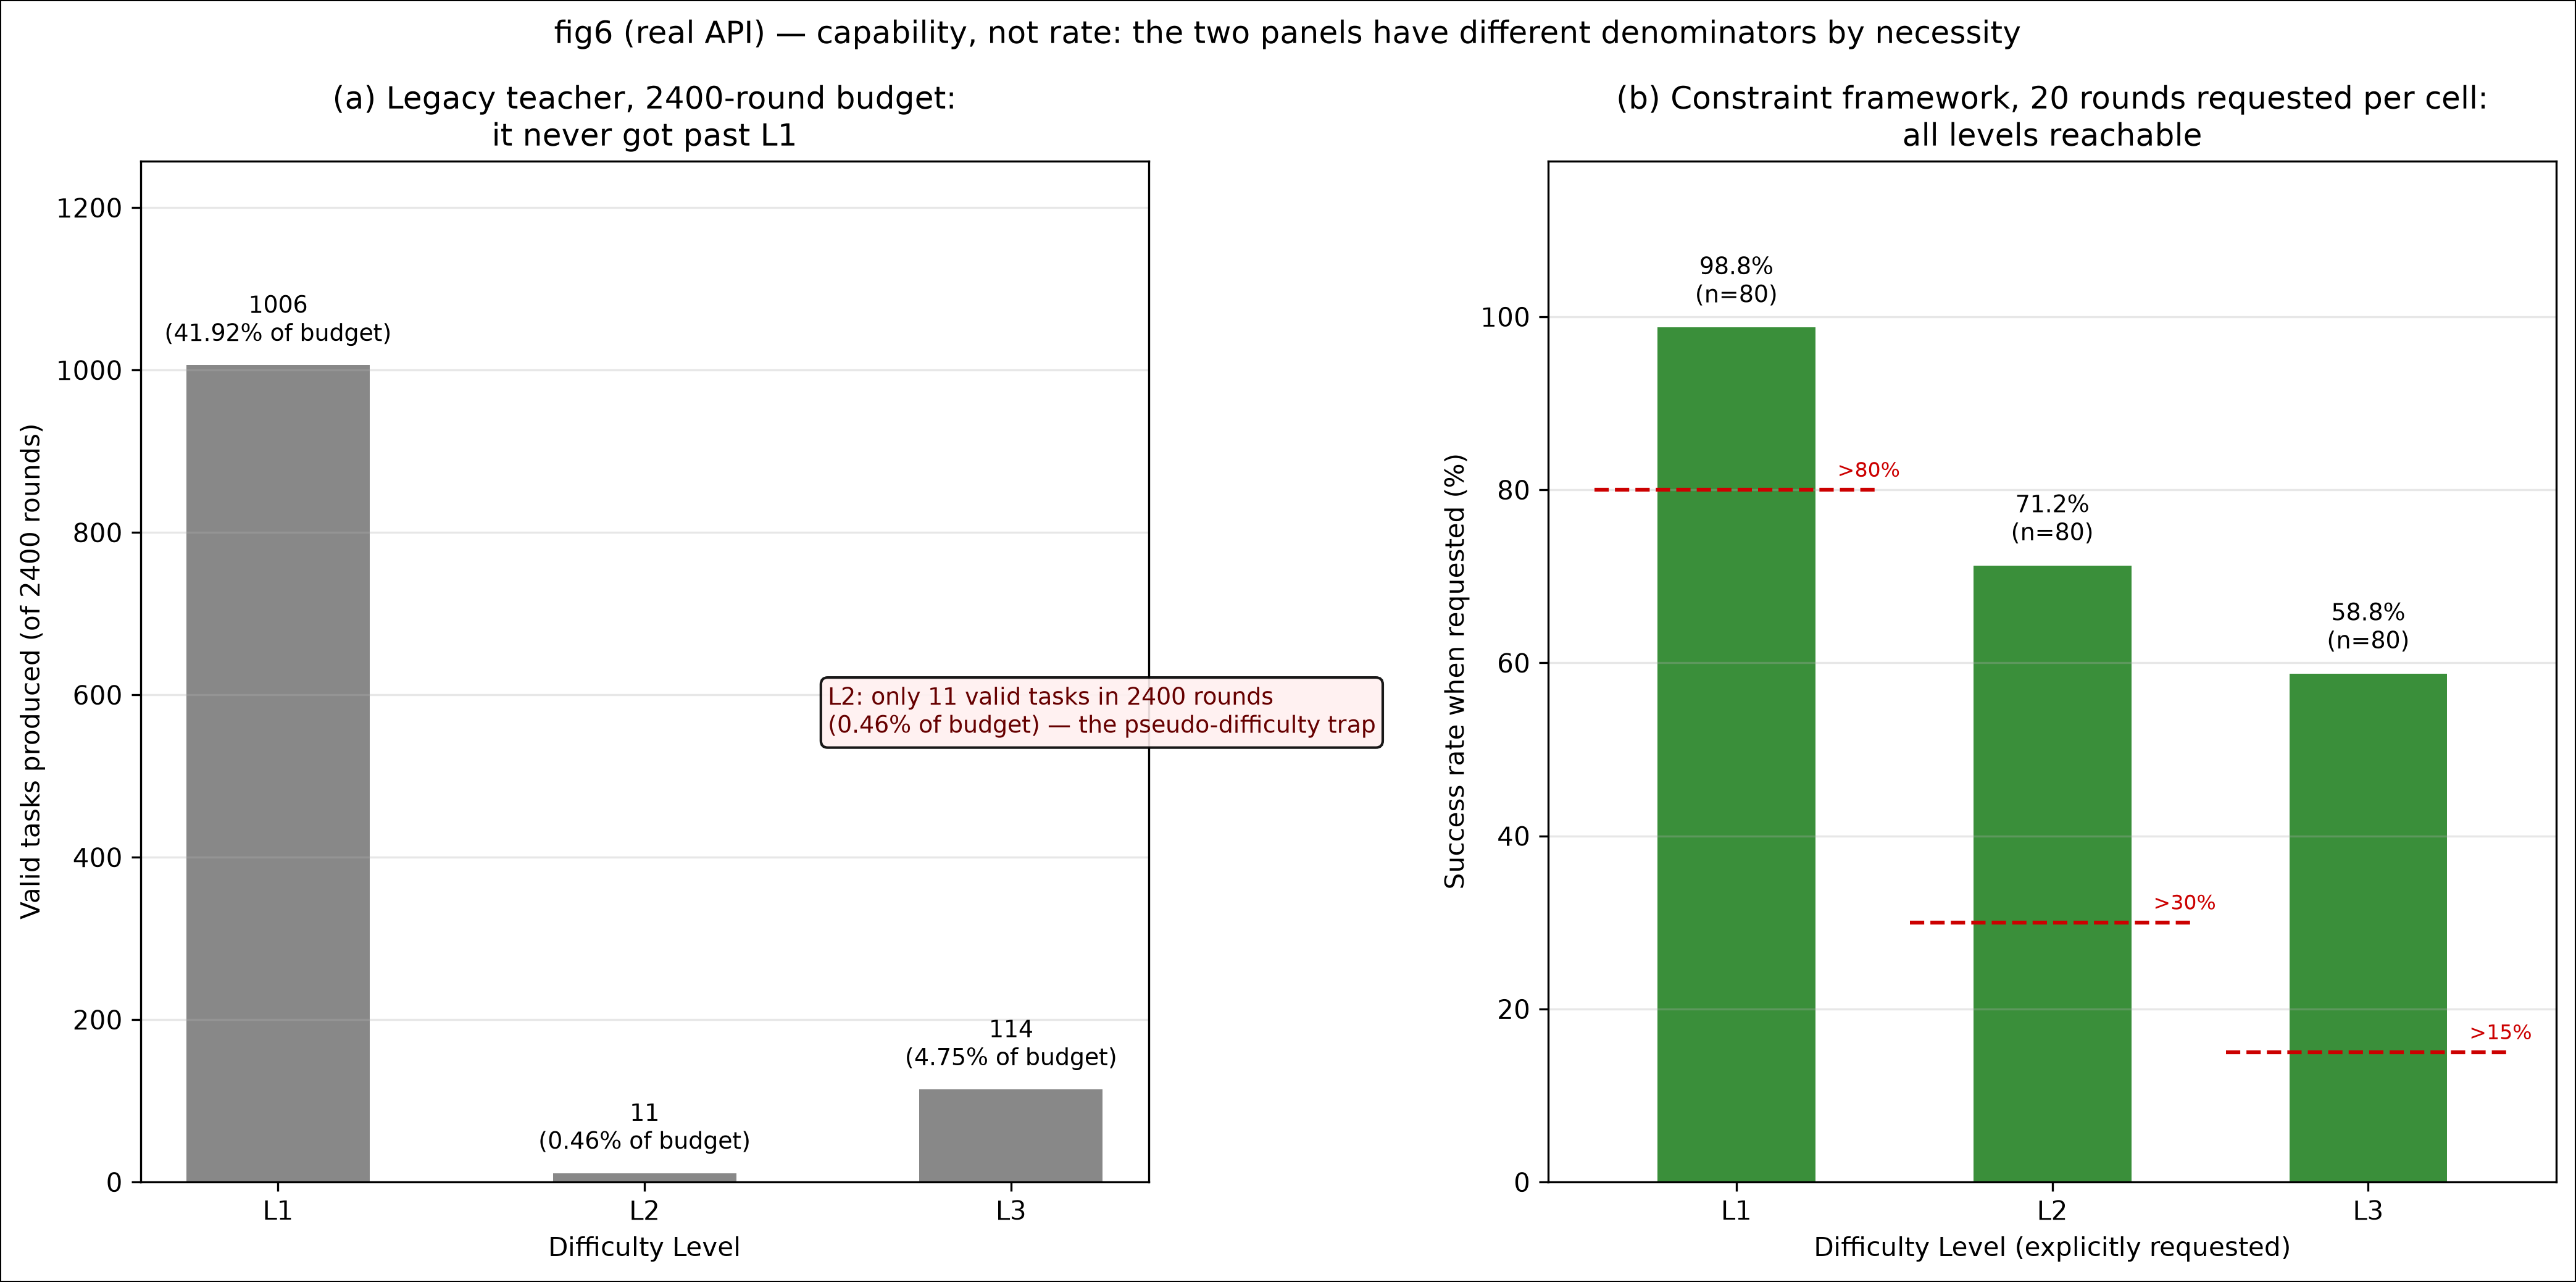
\includegraphics[width=\textwidth]{figures/fig6_improvement_comparison_real.png}
  \caption{Before/after the four-layer constraint generation framework, 240 rounds on the real API
  (4 conditions $\times$ 3 levels $\times$ 20 rounds). Valid-task rate with the framework is L1 =
  98.8\% (79/80), L2 = 71.2\% (57/80), L3 = 58.8\% (47/80); the legacy teacher produced only 11
  valid L2 and 114 valid L3 tasks across 2,400 rounds. Because the two runs differ in budget and
  denominator, this compares capability, not rates.}
  \label{fig:improvement_comparison}
\end{figure*}

\begin{table}[t]
  \centering
  \caption{Constraint framework improvement (real API).}
  \label{tab:table5}
  \small
  \begin{tabular}{@{}lrrr@{}}
    \toprule
    Level & Valid & Total & Valid rate \\
    \midrule
    L1 & 79 & 80 & 98.8\% \\
    L2 & 57 & 80 & 71.2\% \\
    L3 & 47 & 80 & 58.8\% \\
    \bottomrule
  \end{tabular}
\end{table}

% NOTE: fig3b is generated from the legacy 2400-round logs
% (argus-workspace/full/logs/), so its caption documents the failure that
% motivated the framework rather than the post-framework result. Table 5 carries
% the post-framework numbers.
\begin{figure*}[t]
  \centering
  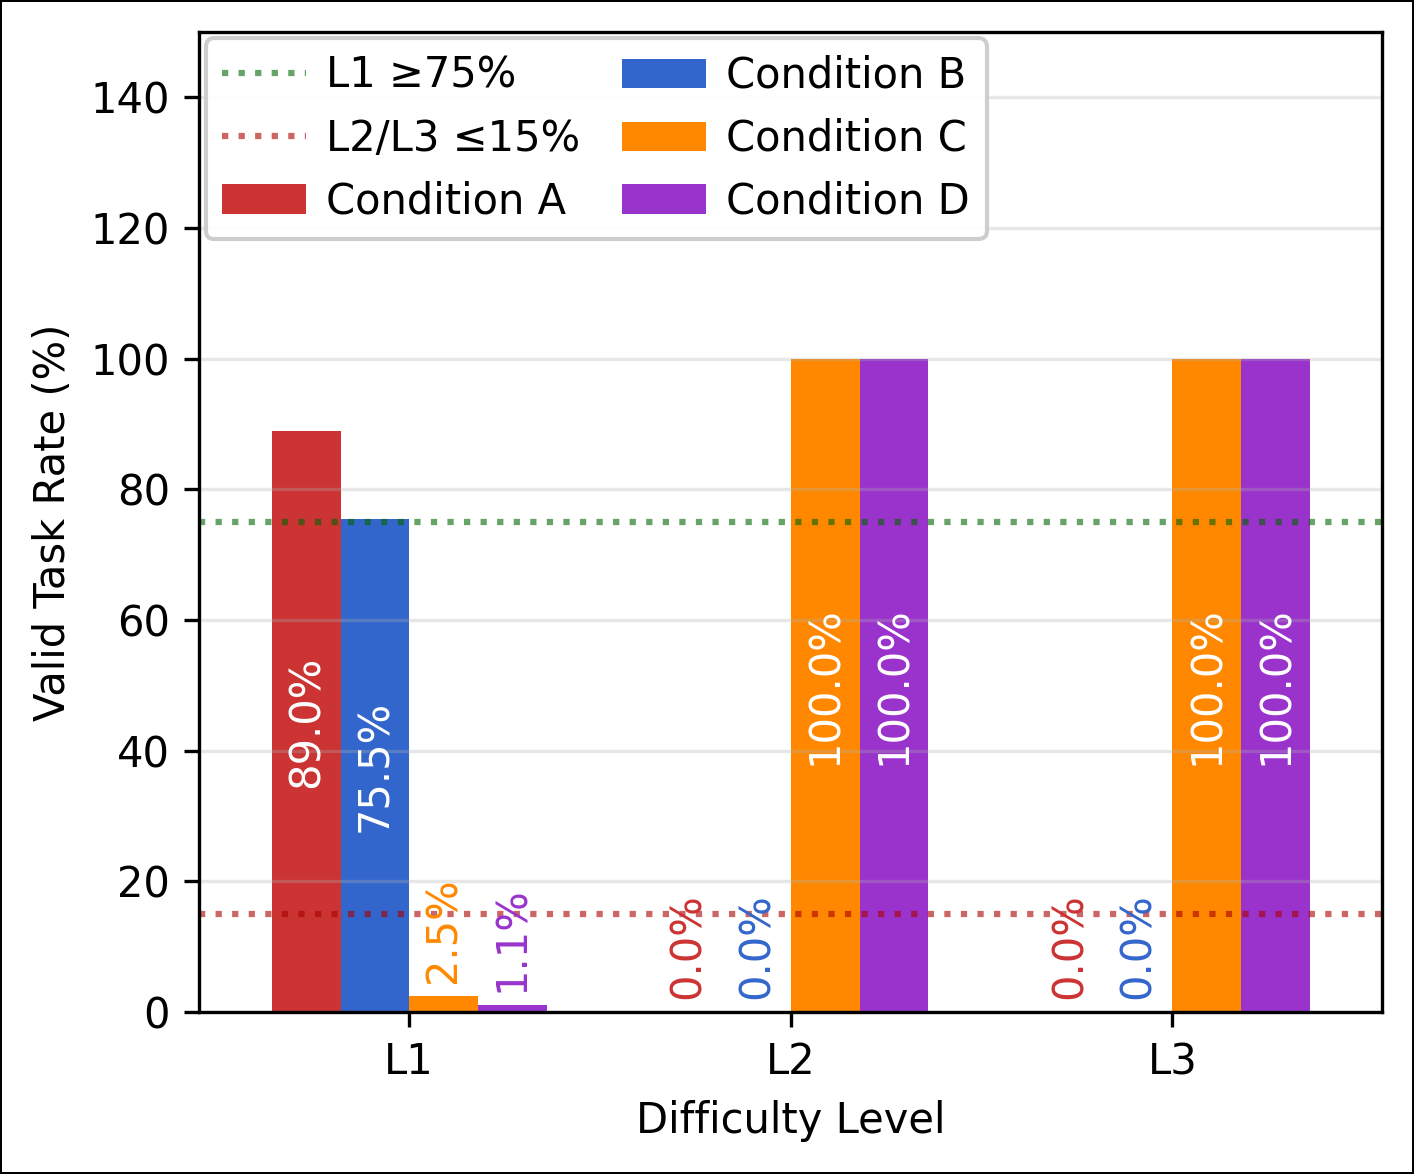
\includegraphics[width=\textwidth]{figures/fig3b_validity_by_level.png}
  \caption{Valid-task rate split by difficulty level. The invalid rate at L2/L3 exceeds 80\% in all
  four conditions, showing that the LLM is unreliable at Z3 constraint generation from L2 upward
  regardless of which mechanisms are enabled.}
  \label{fig:validity_by_level}
\end{figure*}

\subsection{Statistical Validation}

Because the legacy per-level denominators exclude its failed rounds, only the L1 comparison is
caliber-consistent. There the improved teacher shows a lower $\Delta_t$ (0.013 vs 0.082; Welch
$t = 5.43$, $p = 6.0\times10^{-8}$, Cohen's $d = 0.89$, large). Full results and the caliber caveats
are in the released validation report.

% ===========================================================================
% 7-8
% ===========================================================================
\section{Discussion}

The formula implies that ``reliable enough'' is not an absolute property. A 55\%-reliable judge
suffices for a system with $\Delta_t^{\max} = 0.35$. This reframes judge scarcity: the practical
question is not ``can we find a perfect judge?'' but ``what tolerance $\Delta_t^{\max}$ can the
system afford given its generator's $\Delta_t^{\text{gen}}$?''

We derive three concrete pre-deployment checks. (1) Measure the generator's error
$\Delta_t^{\mathrm{gen}}$ at the highest difficulty the controller is allowed to request. If
$\Delta_t^{\mathrm{gen}} \ge \Delta_t^{\max}$, the generator is the bottleneck; improving the judge is
wasted effort. (2) Measure the judge's error on a held-out set of valid tasks; this gives $\tau$
directly. (3) Plug both into $\tau_c = \sqrt{1 - 2\Delta_t^{\max}}$ and compare with the measured
$\tau$. If $\tau < \tau_c$, expect monotone drift; if $\tau \ge \tau_c$, expect stable or improving
behavior. In our case, the L1 sweep returned $\tau = \tau_c = 0.55$, and the L2/L3 regime returned
$\Delta_t^{\mathrm{gen}} \approx 0.9 > \Delta_t^{\max} = 0.6$, correctly predicting the
pseudo-difficulty trap before it was observed in the full 2{,}400-round run.

The composition law also suggests an architectural direction. Self-evolving systems should expose two
measurements as first-class telemetry: a running estimate of $\Delta_t^{\mathrm{gen}}$ per difficulty
level, and a calibrated estimate of $\tau$ per judge. With both available, a controller can decide
per-round whether to escalate difficulty (gated by $\Delta_t^{\mathrm{gen}} < \Delta_t^{\max}$) or to
spend budget on judge calibration. Our four-layer constraint framework is one instantiation of this
idea: it reduces $\Delta_t^{\mathrm{gen}}$ until the generator stops consuming the entire budget, at
which point $\tau_c$ becomes a meaningful operating threshold rather than a constant to be measured.

\section{Conclusion}

We set out to measure how reliable a judge must be for a self-evolving agent to improve. We found
that the answer is not a fixed number. It is a function of how much error budget the generator has
already spent. The composition law
$1 - \Delta_t^{\mathrm{global}} = (1 - \Delta_t^{\mathrm{gen}})(1 - \Delta_t^{\mathrm{valid}})$
holds to machine precision on 2{,}400 real-API rounds, and it implies a closed form
$\tau_c = \sqrt{1 - 2\Delta_t^{\max}}$ with no fitted parameters. The practical consequence is that
``how reliable must the judge be?'' and ``where should I invest?'' are the same question, answered by
the same budget decomposition.

Two results follow. First, the pseudo-difficulty trap: once the generator bottleneck exceeds the
tolerance, no judge reliability can rescue the loop. Second, the judge threshold has a closed form
that holds across mechanisms --- a system with population game, distillation, and
round-table consensus returns the same $\tau_c$ as a minimal Z3-anchored loop. The formula does not
care how many mechanisms you enable; it cares how much budget the generator leaves over. We hope this
reframes the self-evolution problem from ``add more mechanisms'' to ``measure the budget split
first.''

% ===========================================================================
% REFERENCES
% ===========================================================================
\bibliographystyle{plainnat}
\bibliography{refs}

% ===========================================================================
% APPENDICES
% ===========================================================================
\appendix

\section{Complete Figure Gallery}

\begin{figure*}[t]
  \centering
  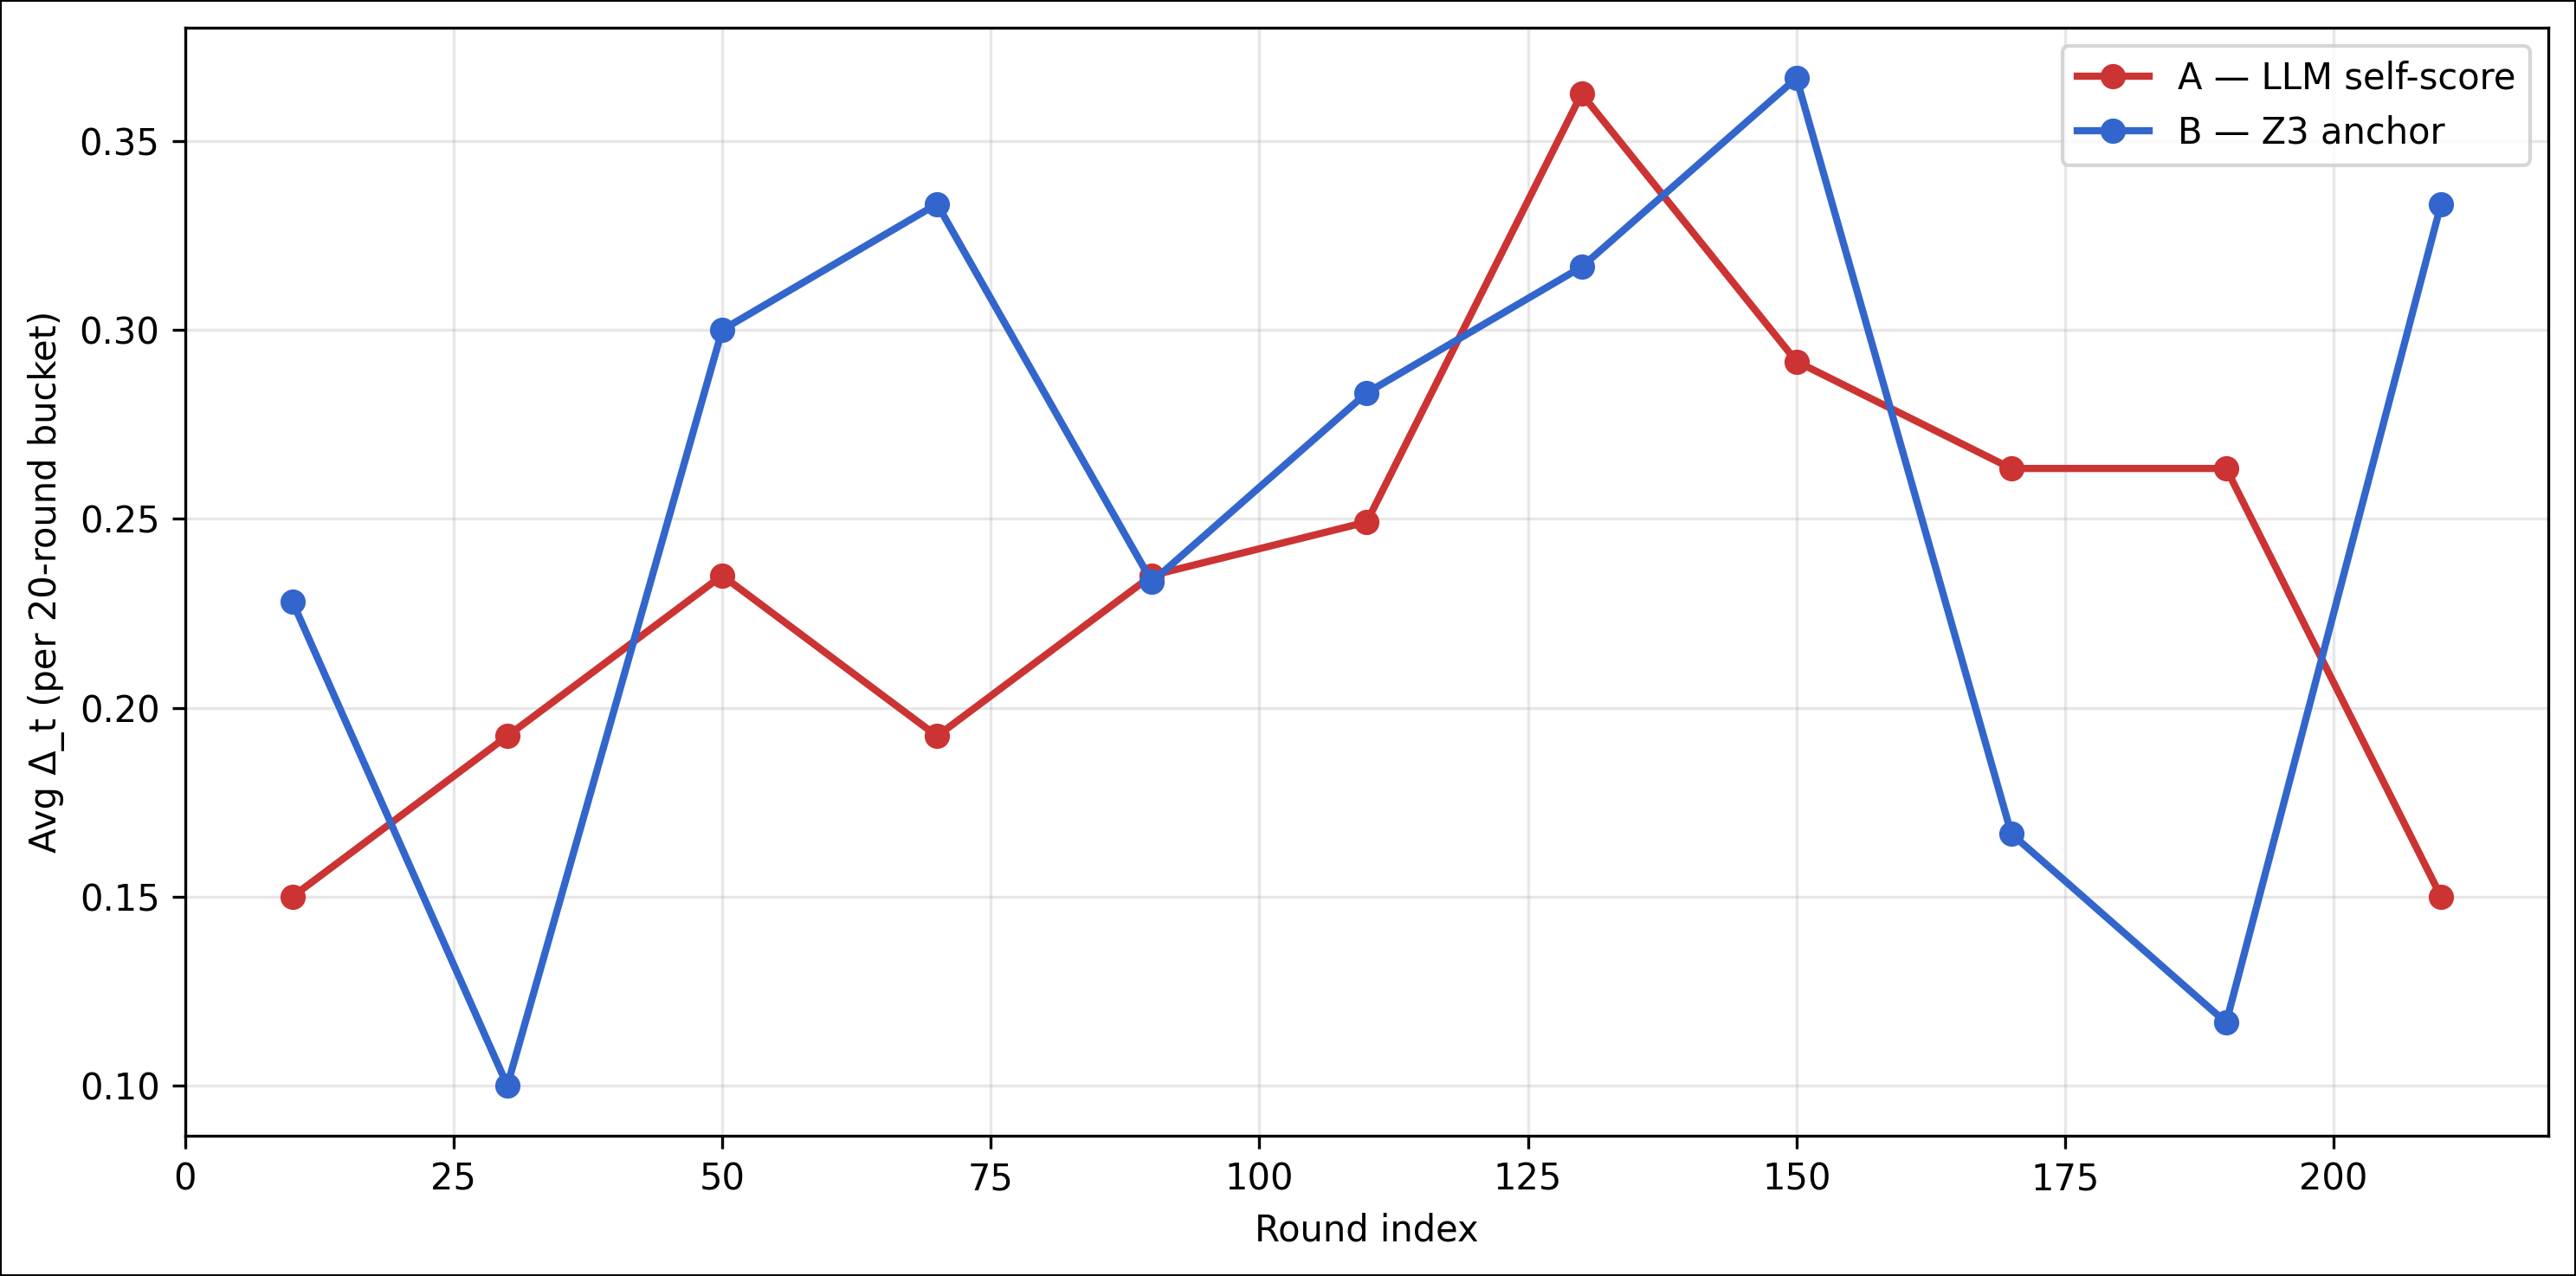
\includegraphics[width=\textwidth]{figures/fig2_delta_t_AB.png}
  \caption{Global-caliber $\Delta_t$ (invalid rounds encoded as $\Delta_t=1.0$).
  Condition A averages 0.2435 and Condition B averages 0.2450---they appear
  similar because B's larger invalid rate offsets its zero valid-round bias.
  The valid-only caliber (Figure~\ref{fig:delta_t_per_round}) isolates judge
  behavior and is the correct view for comparing judge reliability.}
  \label{fig:delta_t_global}
\end{figure*}

\begin{figure*}[t]
  \centering
  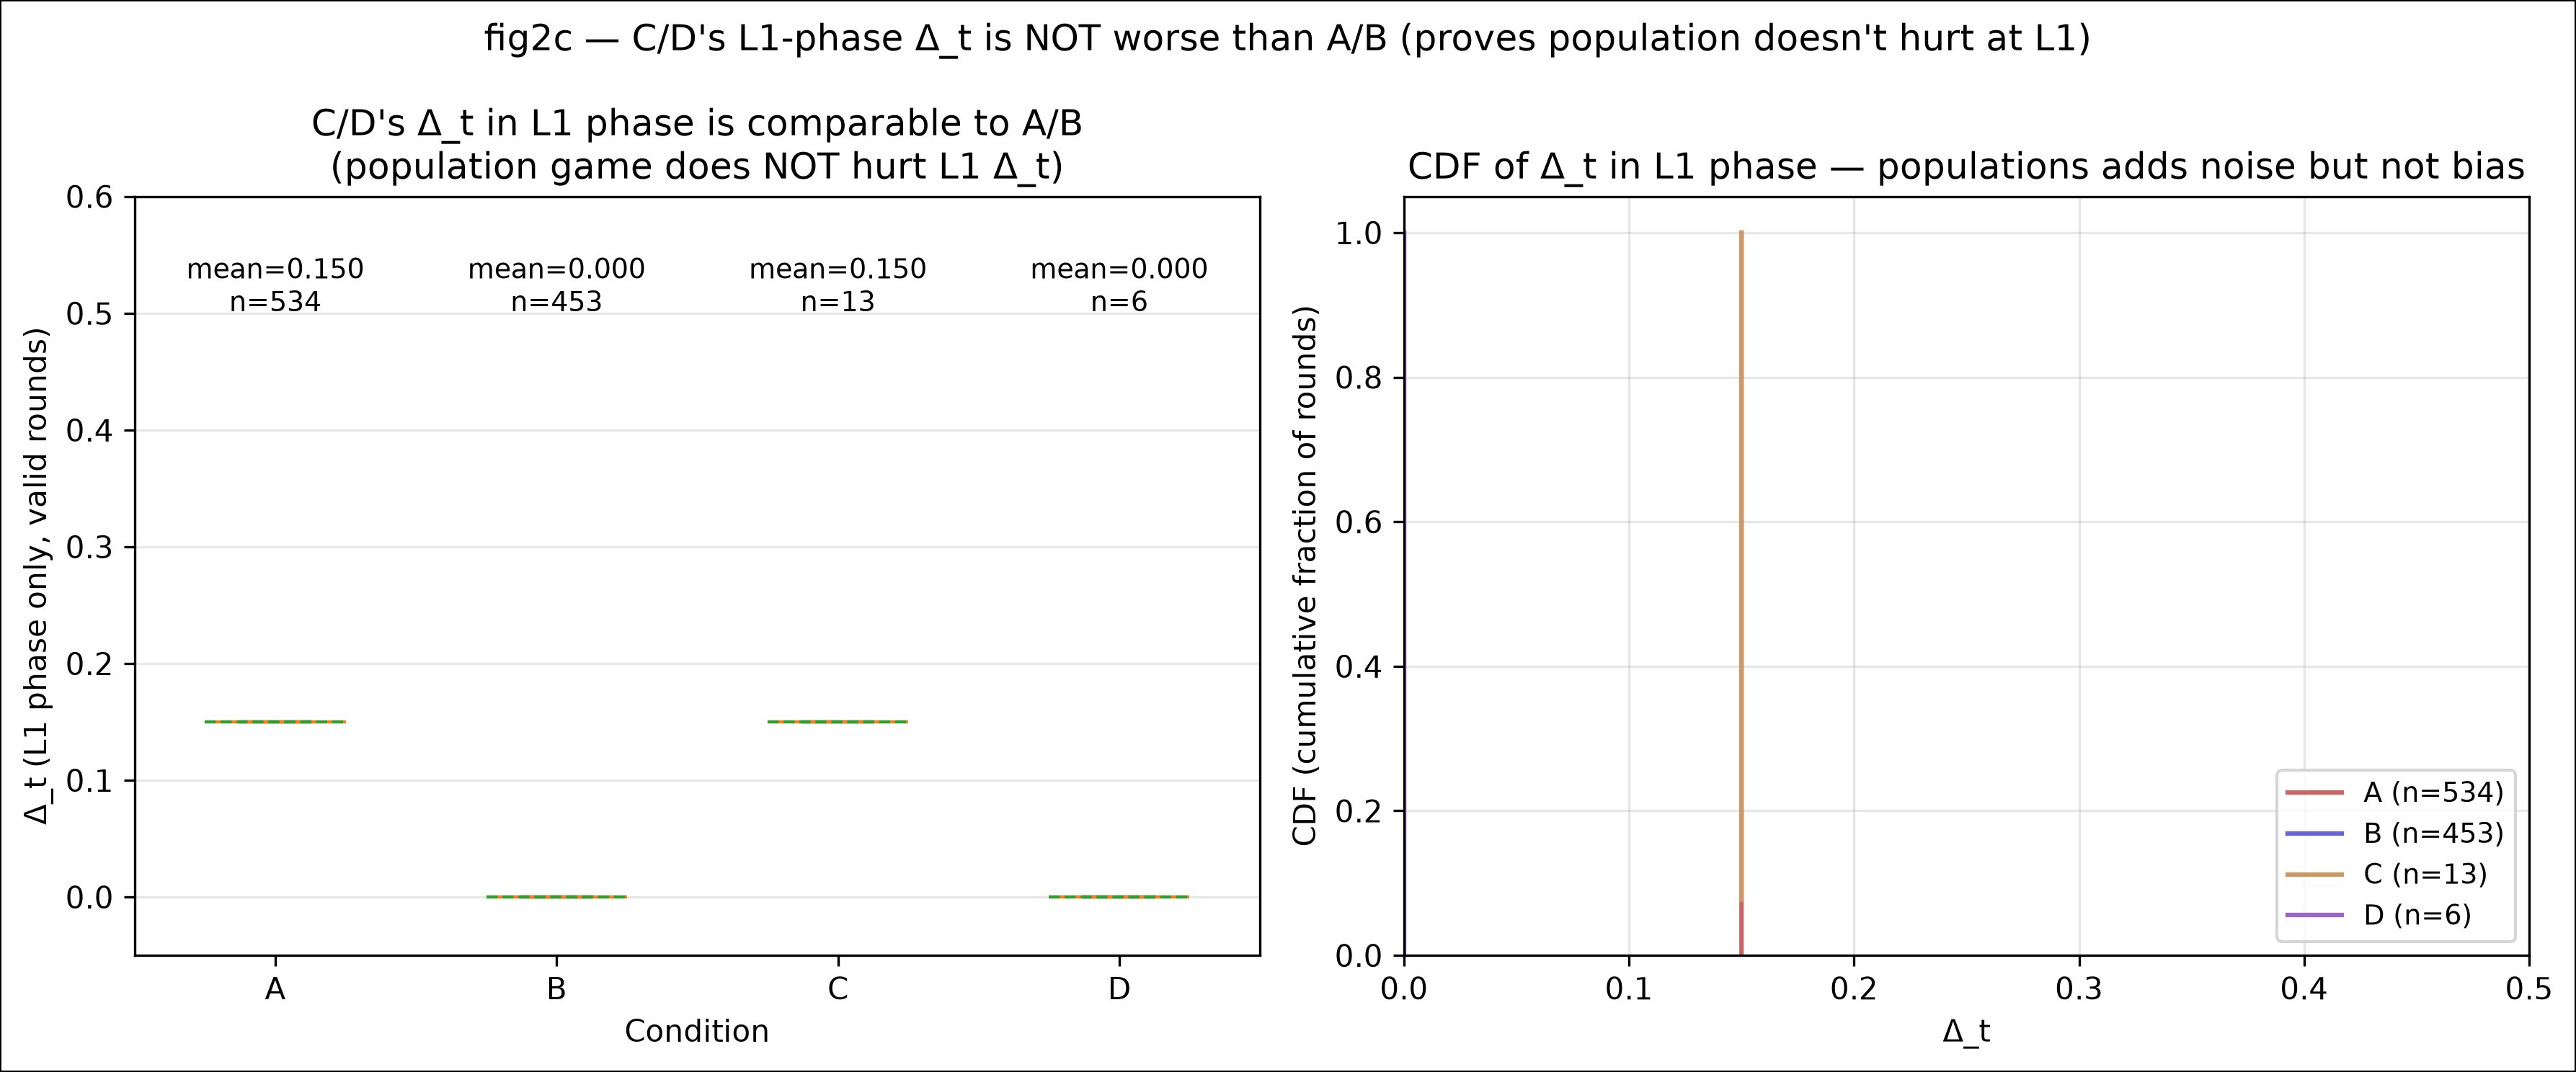
\includegraphics[width=\textwidth]{figures/fig2c_delta_t_L1_only.png}
  \caption{Restricted to the rounds before C/D are promoted to L2. C/D's $\Delta_t$ in the L1 phase
  is \textit{not} worse than A/B, so the population game itself does not hurt performance --- C/D's
  later degradation comes from difficulty escalation, not from a defect in the mechanism. Note:
  C/D's L1-phase sample sizes ($n = 13$, $n = 6$) are small because the difficulty controller
  escalates quickly. The claim ``populations do not hurt at L1'' is directional; a larger-sample
  confirmation is left to future work.}
  \label{fig:delta_t_L1_phase}
\end{figure*}

\begin{figure*}[t]
  \centering
  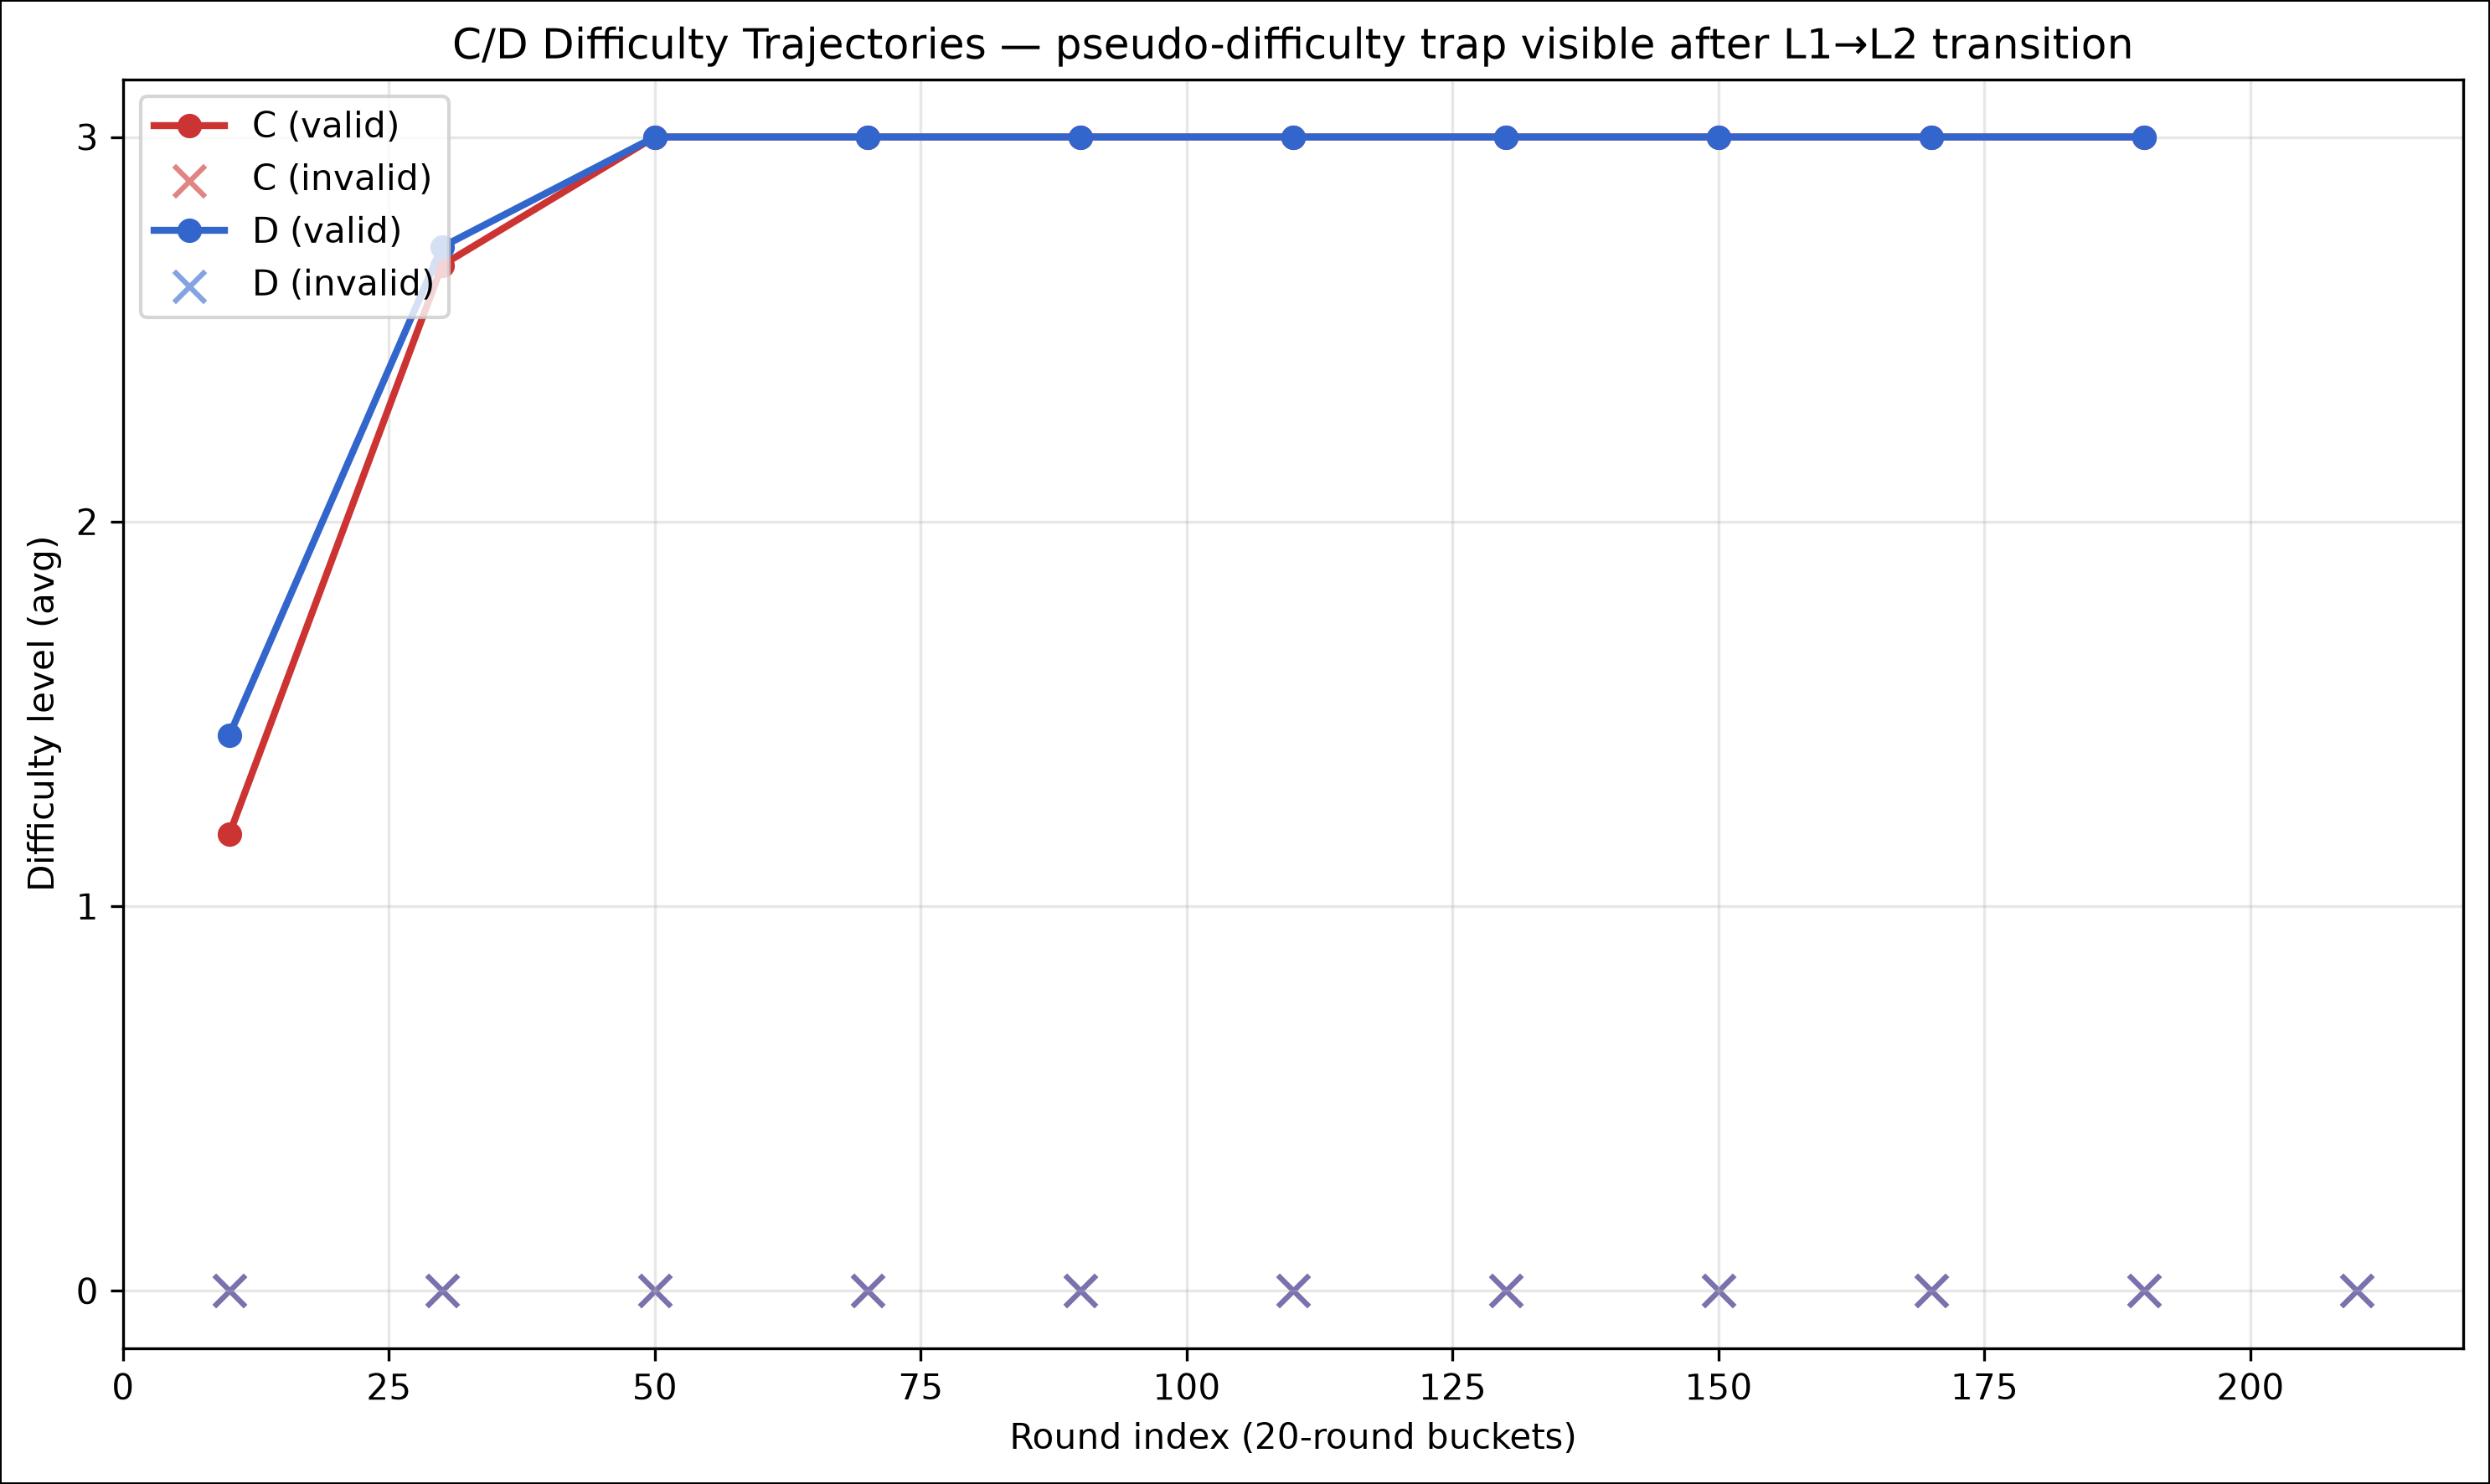
\includegraphics[width=\textwidth]{figures/fig4_difficulty_trajectory.png}
  \caption{Difficulty trajectories for conditions C and D. Failures are \textit{not} distributed
  evenly across difficulty --- they cluster at the moment of escalation. Once the level is raised
  the teacher keeps failing while the controller holds the level high, so the system believes it is
  solving harder problems while actually spending its budget on unusable task proposals.}
  \label{fig:difficulty_trajectory}
\end{figure*}

\begin{figure*}[t]
  \centering
  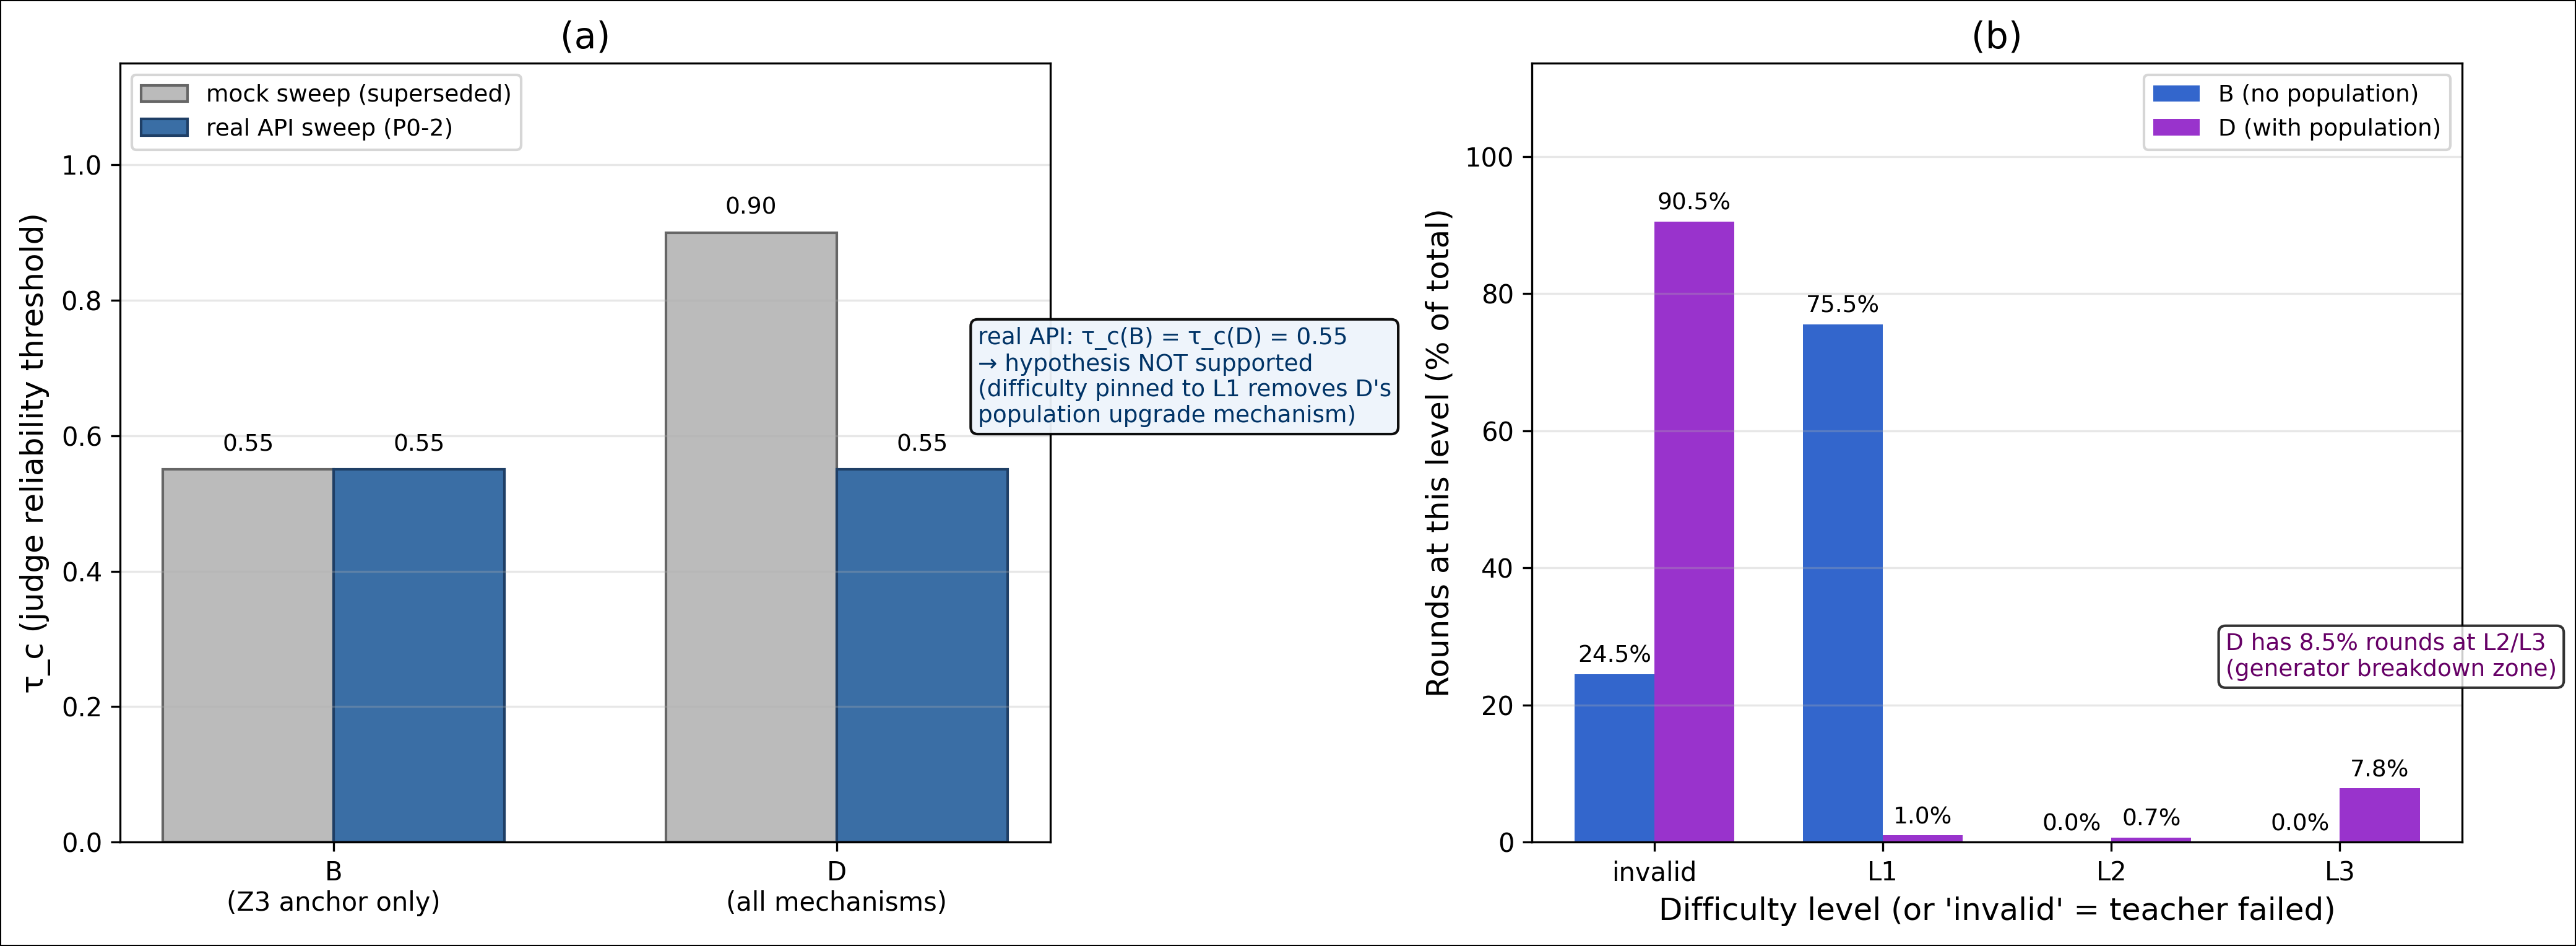
\includegraphics[width=\textwidth]{figures/fig7_tau_c_gap.png}
  \caption{Early mock data reported $\tau_c(B) = 0.55$ versus $\tau_c(D) = 0.90$; the real API does
  not reproduce that gap (both are 0.55). The left panel compares the difficulty distributions of B
  and D, the right panel places the mock and real $\tau_c$ side by side. The original hypothesis
  $\tau_c(D) > \tau_c(B)$ is \textit{not supported}.}
  \label{fig:tau_c_gap}
\end{figure*}

\section{Theorem 1 Proof Sketch}

\subsection*{Algebraic derivation of the composition law}

% NOTE: the brief asks for this derivation under "Appendix B". Appendix B is
% titled "Theorem 1 Proof Sketch" in the agreed structure, so the derivation is
% carried here as a subsection. Rename the appendix if it should stand alone.

Let $S = 1$ if the round succeeds (valid task + correct judgment), $0$ otherwise. Let $G = 1$ if the
generator produces a valid task, $0$ otherwise. Let $V = 1$ if the judge correctly evaluates the
round, $0$ otherwise. Then $S = G \cdot V$. By independence:
\[
  \mathbb{E}[S] = \mathbb{E}[G] \cdot \mathbb{E}[V]
\]
\[
  1 - \Delta_t^{\text{global}} = (1 - \Delta_t^{\text{gen}})(1 - \Delta_t^{\text{valid}})
\]

\section{Rejected Alternative Model}

A simpler account of the same $\tau^{2}$-shaped curve deserves to be stated explicitly, because it is
the most likely competing hypothesis a reader will arrive with. It replaces the second independent
judgment with an acceptance gate: the system accepts the judge's verdict with probability $\tau$ and
otherwise overrides it with its own evaluation, which is itself unreliable. Under that model a round is
correct only when \textbf{both} events succeed, so

\[
  P(\text{correct}) = \tau \cdot \tau = \tau^{2}
  \qquad\Longrightarrow\qquad
  \Delta_t = 1 - \tau^{2}
\]

The three incorrect paths of that model --- judge correct but overridden, $\tau(1-\tau)$; judge wrong
but accepted, $(1-\tau)\tau$; and both wrong, $(1-\tau)^{2}$ --- sum to

\[
  \tau(1-\tau) + (1-\tau)\tau + (1-\tau)^{2} \;=\; (1-\tau)(1+\tau) \;=\; 1-\tau^{2}
\]

\textbf{The discriminating test.} The two models differ by exactly a factor of two on the bias scale,
since $(1-\tau^{2}) \big/ \bigl((1-\tau^{2})/2\bigr) = 2$, and they separate without any fitting.
Section~5.3 compares both against the measured \texttt{correct\_rate}:

\begin{center}
\small
\begin{tabular}{@{}llr@{}}
  \toprule
  Model & $P(\text{correct})$ & MAE vs observed \texttt{correct\_rate} \\
  \midrule
  Two independent judgments (\textbf{this work}) & $(1 + \tau^{2})/2$ & \textbf{0.0389} \\
  Judge $+$ acceptance (rejected) & $\tau^{2}$ & 0.2291 \\
  \bottomrule
\end{tabular}
\end{center}

Over the 16 $(\tau, \text{condition})$ cells the two-judgment model is closer in 13, tied in 2 and
loses in 1. The rejection is therefore not a preference between two equally good fits: the acceptance
model is worse by a factor of six in MAE.

\textbf{Why the factor of two appears.} The acceptance model has no \textit{both-wrong} agreement
path. In Section~5.3 a round is scored correct whenever the two verdicts \textbf{agree}, so the
probability mass splits into three exhaustive paths: both unflipped, exactly one flipped, and both
flipped. The first and the third agree with each other and contribute zero error; only the middle
path, of probability $2p(1-p) = (1-\tau^{2})/2$, carries bias. The acceptance model instead charges
the both-wrong case as an error, and that is what doubles $\Delta_t$. The exponent of $\tau$ is fixed
by the number of independent judgments the system requires to agree --- a property of the
architecture, not of the judge.

At the grid's lower edge, $\tau = 0.55$, the rejected model predicts $\Delta_t = 1 - 0.55^{2} =
0.6975$, against a measured 0.3000 (B) and 0.3200 (D) and a closed-form prediction of
$(1 - 0.55^{2})/2 = 0.3488$. At the boundary $\tau = 0.5$ the rejected model gives $\Delta_t = 0.75$
against $0.375$ from the closed form --- a clean factor of two, though the swept grid begins at
$\tau = 0.55$ and therefore holds no measurement at that point. \textbf{No result in this paper uses
$\Delta_t = 1-\tau^{2}$.}

\section{Data Consistency Check}
\label{app:data_consistency}

\setcounter{table}{0}
\renewcommand{\thetable}{D.\arabic{table}}

\subsection{Unified definition of $\Delta_t$}

\[
  \Delta_t \;=\; \bigl| \text{score}(y) - \text{label}(y^{*}) \bigr|
\]

\begin{itemize}
  \item $y$: the round's submitted answer (\texttt{z3\_result.status});
  \item $\text{score}(y)$: the system's normalised score for that answer, in $[0, 1]$;
  \item $\text{label}(y^{*})$: the ground-truth label (\texttt{sat} $= 1.0$, \texttt{unsat} $= 0.0$).
\end{itemize}

\subsection{Source of the system score by condition}

Table~\ref{tab:table2c_sources} records, for each condition, which quantity plays the role of the
system's evaluation and which plays the role of ground truth.

\begin{table*}[t]
  \centering
  \caption{Where the system score and the ground-truth label come from in each condition. In B and D
  the Z3 verdict is compared against itself, so $\Delta_t$ is identically zero on every valid round;
  the global caliber of Section~\ref{subsec:calibers} is what reintroduces a non-zero average.}
  \label{tab:table2c_sources}
  \small
  \begin{tabularx}{\textwidth}{@{}l l l >{\raggedright\arraybackslash}X@{}}
    \toprule
    Condition & System score $\text{score}(y)$ & Ground truth $\text{label}(y^{*})$ & $\Delta_t$ \\
    \midrule
    A & \texttt{llm\_self\_score} (LLM self-score) & \texttt{expected} (Z3 truth) &
        $\bigl|\texttt{llm\_self\_score} - \text{truth}\bigr|$ \\
    B & \textbf{Z3 anchor} $=$ \texttt{z3\_result.status} & \texttt{expected} &
        \textbf{0.00} --- the Z3 verdict adopts the truth directly, so it is compared with itself \\
    C & \texttt{llm\_self\_score}, averaged over the population & \texttt{expected} &
        $\bigl|\texttt{llm\_self\_score} - \text{truth}\bigr|$ \\
    D & \textbf{Z3 anchor} $+$ round-table consensus & \texttt{expected} &
        \textbf{0.00} --- the Z3 verdict is self-consistent \\
    \bottomrule
  \end{tabularx}
\end{table*}

\subsection{Two statistical calibers}
\label{subsec:calibers}

\textbf{Caliber 1: valid-only $\Delta_t$ (Table~\ref{tab:table2b}).} The denominator is
\texttt{len(records[r.valid])}. Invalid rounds --- those in which teacher generation failed and no
ground-truth label exists --- are excluded. Under this caliber A gives $\Delta_t \approx 0.15$, since
the LLM self-score deviates from the Z3 truth on a small number of rounds, while B and D give
$\Delta_t \equiv 0.00$, because the Z3 verdict is compared against itself.

\textbf{Caliber 2: global $\Delta_t$ (this appendix and Figure~\ref{fig:delta_t_global}).} The
denominator is all rounds. Invalid rounds are encoded conservatively as $\Delta_t = 1.0$ and valid
rounds keep their valid-only value. Under this caliber A rises to $\approx 0.24$, moved by the $11\%$
invalid rounds, and B rises to $\approx 0.25$, moved by the $24\%$ invalid rounds.

\subsection{Resolution of the apparent contradiction}

A reader comparing the two reports will find A $= 0.15$, B $= 0.00$ in one and A $= 0.2435$,
B $= 0.2450$ in the other. These are \textbf{not} in conflict: they are the same rounds read under
the two calibers above, and Table~\ref{tab:table2c_calibers} verifies both simultaneously.

\begin{table*}[t]
  \centering
  \caption{The same rounds under both calibers. The valid-only rows are the entries of
  Table~\ref{tab:table2b}; the global rows additionally charge every invalid round $\Delta_t = 1.0$.}
  \label{tab:table2c_calibers}
  \small
  \begin{tabular}{@{}llrr@{}}
    \toprule
    Caliber & Condition & $n$ & Avg $\Delta_t$ \\
    \midrule
    valid-only & A & 534 & 0.1500 \\
    global     & A & 600 & 0.2435 \\
    valid-only & B & 453 & 0.0000 \\
    global     & B & 600 & 0.2450 \\
    valid-only & C & 87  & 0.1879 \\
    global     & C & 600 & 0.8823 \\
    valid-only & D & 57  & 0.0000 \\
    global     & D & 600 & 0.9050 \\
    \bottomrule
  \end{tabular}
\end{table*}

The paper uses \textbf{caliber 1 (valid-only)} for its main tables, and \textbf{caliber 2 (global)}
when describing the pseudo-difficulty trap, where the quantity of interest is precisely how many
rounds C and D invalidate.

% ---------------------------------------------------------------------------
% UNPLACED FLOATS
%
% The published data package holds 9 tables. Seven now have a home (table4c
% supplies two of them); these two still need one. Move each into the section
% that should cite it and give it a \caption and a \label.
%
%   table2a_delta_t_global        global caliber (discussed in 4.2)
%   table4b_analytical_fit        per-tau residuals (discussed in 5.3)
%
% NOTE: table2c_delta_t_semantics is now placed in Appendix D as
% \ref{tab:table2c_sources} and \ref{tab:table2c_calibers}; that is what the
% Section 4.2 pointer \ref{app:data_consistency} resolves to.
%
% NOTE: table4c is now placed in Section 4.1 as \ref{tab:table4c}, with its
% budget-decomposition part as \ref{tab:table4cbudget} in Section 4.4.
% ---------------------------------------------------------------------------

\end{document}
